
\chapter{Reference Model Construction}
%%%%%%%%%%

This chapter conceptions the process reference model and is central part of this thesis. In order to discuss particular processes, the framework itself needs to be discussed. What follows is the discussion of processes, which puts special emphasis on design decisions, \viz \textit{how} to model certain aspects by means of the language icebricks. 

	%%%%%%%%%%
	deloitte W14: managing change dispute:::: innovation und so... wichtig für begründung des frameworks
	\section{Process Framework}
	
	\citeauthor{Meise2001} defines a framework as \enquote{an ordering of relevant elements and relationships on a high level of abstraction. [...] Purpose is to give an overview about an original and to support structuring of elements and relationships on lower detail levels} \citep[\p{62}]{Meise2001}. Drawing further on his work, which especially targets framework design in process-oriented organizations, the proposed procedure for construction is adopted (\Fig \ref{fig:meise}). Differences to his approach arise, as the reference model displays an as-is state of the domain and does not follow goals of reorganization set by a specific company. Therefore, the \textit{organization} represents a fictive BPO provider in CRM in the following, which captures generic aspects of the domain. The construction is split into two components. The structural part first encompasses strategic and fundamental reflections, while the graphical component transfers these into a visual form that supports communication.

	\begin{figure}[caption={Procedure for framework construction}, label={fig:meise}]
		{	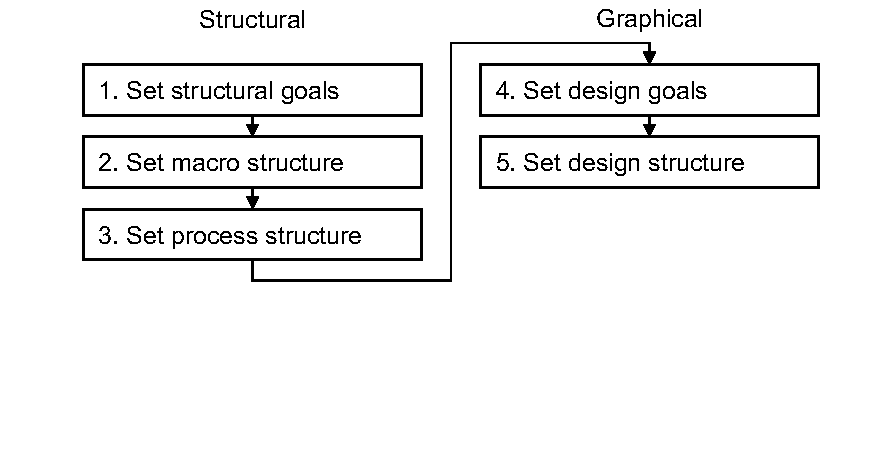
\includegraphics[width=.8\textwidth]{figures/framework-meise.pdf}}
		\parbox{0.7\textwidth }{\quelle{Adapted from \citep[\p{122}]{Meise2001}}}
	\end{figure} 
	
	\subsection{Set structural goals}
	
	Modeling is no end in itself and different purposes require different models. Theoretically speaking, purpose of this research is to create an artifact that generates utility and tackles a problem in the real-world.  Previously identified problems (\ref{sec:proide}) lead to objectives (\ref{sec:solobj}) which are to be faced with the process reference model in general and its framework in particular. The existence of general (organizational) and stakeholder-related objectives requires the framework to bring together both ends.
	
	\begin{table}[caption={Solution Objectives}, label={tab:solobj}]
		\centering
		\begin{tabular}{l p{13.3cm}}

			\textbf{No. }&\textbf{ Solution Objective}
			 \\ \hline
			\textbf{1 }                        & Construction of a generic reference model that covers distinguishing processes for BPO-providers in CRM on concept level.                                                    \\ \hline
			\textbf{2}                         & The reference model can be applied for use at Arvato CRM.                                                                                                                    \\ \hline
			\textbf{3 }                        & The construction,process is well-documented, makes use of empirical research by induction, which is enriched by deduction from \acrshort{BPO} and \acrshort{CRM} theory. \\ \hline
			\textbf{4}                         & A syntactic and semantic formalized process modeling language is used, that is transferable to other languages.                                                              \\ \hline
			\textbf{5}                         & The model can be used as a statement of competence for sales activities towards clients.                                                                                     \\ \hline
			\textbf{6}                         & The model holds a process representation, which supports a common understanding across client businesses.                                                                    \\ \hline
			\textbf{7}                         & The model is able to represent an omni-channel environment.                                                                                                                 
		\end{tabular}
	\end{table}

	
	
	\subsection{Set macro structure}
	
	A framework, as a strategic tool, incorporates concepts of strategy. One can name two perspectives, namely a market- or resource-based view of strategy, which are directed externally or internally, respectively. They are not independently of each other, but their interplay is seen as an important factor in strategic decision making. Literature criticizes that standardization through reference model application has contra-productive effects on strategic competitive advantages. \cite{becker2004handelsinformationssysteme} note that the argument is true, when the reference model is used as an application model. However, the application of the reference should incorporate strategic characteristics of the company. This reference model framework is designed in a way that generic strategic orientation for providers is incorporated. 
	
	The market-based view follow the structure-conduct-performance paradigm, that explains success of a company through external factors in the industry. \cite{porter1980} formulated the so called five-forces model, which describes bargaining power of suppliers (1), threat of substitutes (2), bargaining power of buyers (3), threats of new entrants (4) and industry rivalry (5) as determinants of competition. Applying these two the BPO domain, a trivial substitute for outsourced services is the return of services inside the parent organization. Further, the substitution of customer services through automation may render outsourcing obsolete. The bargaining power of suppliers and buyers can be loosely mapped to clients and customers. While clients as suppliers clearly influence the provider directly, customers show less of this influence on the outsourcing provider. As the provider takes an intermediate position between client and customer (\cf \Fig \ref{fig:bpochain}), their acting is always in connection with the client. However, an assessment of outsourced service quality puts pressure originating from the customer on the provider, which in turn will also be judged by the client. The entry of new players on the market (4) can be tackled by barriers, that go back to competitive advantages of differentiation or cost-leadership. While the latter is especially causing fierce competition in low-wage regions that realize offshore-outsourcing, outsourcing players in CRM that feature more profound services, lean towards a differentiation strategy. This can also be stated for Arvato. Lastly, industry rivalry among players in the BPO CRM market is also influenced by the aforementioned generic strategies, to position established companies. A framework adopts market-based aspects through accounting for markets or segments therein. These are accompanied by business units or processes that relate to this external environment. 
	
	The resource-based view of strategy \citep{wernerfelt1984resource} analyzes internal strengths and weaknesses. Resources are bundled to form capabilities and should be rare, inimitable, create value and be non-substitutable. Due to asymmetries of resources, competitive advantages are enabled. The identification of capabilities of CRM BPO providers (\cf \ref{sec:bpocrmis}: operational and business development capabilities) can only be done on a generic level for the reference model. Application necessitates specifying the framework to conform to company-specific capabilities. The operational capability should reflect the operational process component in CRM (\cf \ref{fig:crmprocessfr}), and service delivery from the outsourcing side (\cf \ref{app:provproc}). Business development, \ie understanding and addressing client needs, misses a pendant in an isolated CRM view, but can be put in relation to delivery management in the outsourcing model. 
	
	Putting both views together emphasizes the client and customer market environment and two capabilities, that relate to these markets. Towards the client side, providers are criticized by clients for being too reactive instead of proactive (49\%), delivering poor service quality (48\%) and lack of innovation (37\%) \citep{deloitte2014outsourcing}. While the first point of criticism addresses the client relationship, the other two are directed towards the service itself. Looking at the constituents of \acrshort{CRM}, the people, process, technology split draws a line to the resource-based view, as these three resources need to be developed and captured to enable superior service provision for clients. Apart from the  \acrshort{CRM} view, these three also have their own meaning in \acrshort{BPO}. \todo{Gross} The importance of processes in  \acrshort{BPO} is obvious. The people component can be interpreted here as the provision of manpower and their training for services; (information) technology as an enabler of outsourcing (\cf \ref{sec:bpo}) . 
	
		
	\subsection{Set process structure}
	\label{sec:procstr}
	Given that the model shows processes, the structural split of people, processes and technology is hardly meaningful, as two aspects of  \acrshort{CRM} or \acrshort{BPO} would be left out. Drawing from the BPO chain and the identified stakeholders enables another categorization that leaves room for design choices, while capturing generic aspects of business processes within \acrshort{BPO}. As \acrshort{BPO} is the framing construct and  \acrshort{CRM} one use of it, this order is to be prioritized. The following briefly describes business processes, that are detailed in the remainder of this chapter.
	
	
	\begin{figure}[caption={BPO chain provider scope with stakeholders}, label={fig:bpochainscope}]
		{	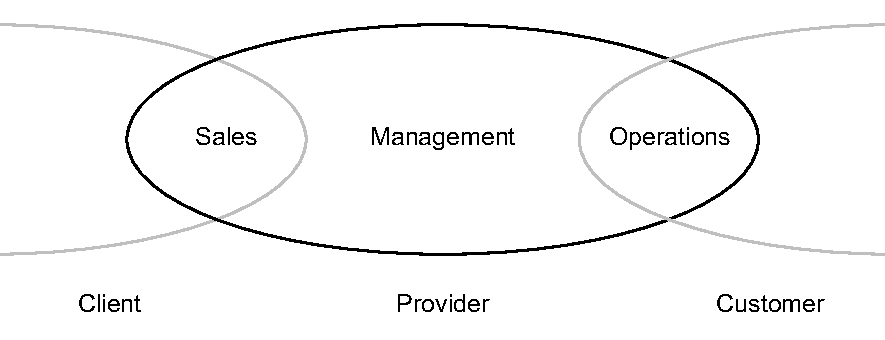
\includegraphics[width=.8\textwidth]{figures/chain2.pdf}}
	\end{figure} 
	
	\subsubsection{Sales-related}
	Sales-related business processes cover processes that have touchpoints with the client. These take place along a lifecycle, which starts with initial contact between provider and client, and hopefully advances through creation of an outsourcing contract. For this agreement, the \acrshort{BPO} provider places its products (\ie, service blueprints) in the clients requirements profile to create solutions for identified problems. Also, the transition and setup of the outsourced business must take place. After everything is set up, the client relationship is maintained under the umbrella of account management. 
	
	\subsubsection{Management-related}
	The management-related business processes bring together resources in the provider organization, so that the operations and business development capability are realized. Regarding the latter, it is important to have a products in place, which can be implemented as service solutions for clients.  \citep{schewe2007} names this delivery management, but explicitly refers to its similarities with product development. In addition to the development, the management of existing products inside a product portfolio becomes important. 
	
	Benefits through economies of scope are a question of offered services and not processes. The operations capability can be addressed by processes, that enable economies of scale. These are realized by the increased output of services across client businesses, which in turn necessitates alignment in these services so that their output can be counted \textit{together}. This alignment is facilitated through a product-view of services and their underlying portfolio in the organization. In addition, people in the provider organization need to be trained  in order to excel in the role of \acrshort{CSR}. Their career path can be seen from a process perspective, so that a strong relationship is established with their employer. This aspect shall be called People Lifecycle Management\footnote{The term people is preferred over agent or \acrshort{CSR}, because it puts this process strongly in connection \acrshort{CRM}. As the management-related processes are tried to be references for \acrshort{BPO} in general, this is not intended.}.  Lastly, management of the workforce, especially scheduling, becomes critical in a business like customer service. The assurance of the right capacity at the right time to meet fluctuating demand with little waiting time is expected from the client. Therefore, efficient techniques to manage the complexity of multiple channels, different demand patterns and different skilled \acrshort{CSR}s are necessary. This is encapsulated in the process of workforce management. 
	
	\subsubsection{Operations-related}
	The last group of business processes target the service delivery in the words of \citeauthor{schewe2007}. The processing of transactions with customers is in focus, which can be on numerous channels. A transaction in this case is a conversation, so that theories of communication \citep{shannon1949} may be used here.  A message is sent from a sender to a receiver through a medium. In case of customer service, both the customer or the \acrshort{CSR} can start a conversation, that has a subject which relates to the client in some way. Reasons for contact may be separated by being related to a previous transaction. This transaction might be a purchase of a client's good or service. The communication channel increasingly varies and is no reasonable split \todo{was für 1 split}, as in an omni-channel environment a seamless experience across channels is intended. Hence, the processes should be similar on a high level of abstraction. 
	
	Communication can be asynchronous (\eg, e-mail) or synchronous (\eg, voice), which puts emphasis on temporal differences in the conversation. While the employed process definition encompasses the \enquote{time-logical sequence of activities}, the value (\viz time between activities) does not impact the process logic itself, as this is a question of succession. General steps in inquiry handling from a business perspective will be similar independent of the (a)synchronous case. What becomes more important from a business perspective is the question after the contact initiator. A communication triggered by the customer (incoming) follows demand patterns that are inferred from historic data, while better planning of \acrshort{CSR} opened contacts (outgoing) is possible, as the temporal decision of contact lies at the business and not the customer. 
	
	Lastly, one has to differentiate in customer contact whether \acrshort{CSR}s are involved in inquiry handling, which obviously has business implications. When customers use self-service to address their needs, software takes the \acrshort{CSR} role, which saves resources. Providers can differentiate themselves through expertise in these systems. Clients save money by less volume that is processed by humans (employees of the outsourcing provider). At first sight, this may cannibalize outsourcing business, but the expertise of installing and running these self-service systems is likely not located in clients that outsource \acrshort{CRM}. Consequently, providers can generate new business by accumulating know-how in self-service activities. On the one hand, they design the customer-facing self-service in order to handle the inquiry (which by definition are customer-initiated). On the other hand, the provider manages and maintains the knowledge base, that sits behind these automatons in the back-end. This knowledge management does not only have implications on self-service, but also on other customer contacts, as the \acrshort{CSR}s in the human-to-human communication also query the knowledge base to solve customer problems.  
	
	It is desisted from the explicit modeling of a customer journey, because it encompasses components that cannot be part of a process model for providers. The model in this thesis is centered on the outsourcing provider. Modeling of a customer journey requires a customer-centric model, which then contains steps of the customer journey in a detailed way. Such a model should be a \textit{playground} for identifying space for improvement in dialog with a client regarding its customer journey. In addition, it would benefit from avoiding the standards of process models, as its purpose is seen in the \textit{design} of a journey through \acrshort{CRM} components. Research from the field of marketing can be a starting point \citep{Lemon_2016, Frow_2007}. 
	
	\subsection{Set design goals}
	
	The visual representation of the framework is linked to its cognition among viewers, therefore it needs to support the communication of the reference model's purpose. In contrast to language-processing, the process of perception is foregrounded, as the graphic is processed all at once and not sequentially. The model has to capture the fundamental characteristics of the domain of outsourcing at first glance. The sketched model level when applied (provider and client model) should be visually supported, as the framework of the reference is the blueprint to convey this hierarchy. 
	
	\hfill\begin{minipage}{\dimexpr\textwidth-1.2cm}
		\textbf{Design Goal 1}: The framework has to visualize the business of BPO providers.
	\end{minipage}

From a process perspective, as well as to reduce complexity, it helps to highlight important business processes over supporting or coordinating processes. By doing this, the viewer gets an impression about central parts of the model. 

	\hfill\begin{minipage}{\dimexpr\textwidth-1.2cm}
	\textbf{Design Goal 2}: The framework has to distinguish business processes from other process types. 
\end{minipage}

Furthermore, provisioned services are to be shown. In order to gain an understanding of characteristics in CRM outsourcing, especially in an omni-channel context, the framework has to clearly communicate their orientation towards the customer. As it is the differentiating aspect towards BPO for other processes, this fact could be incorporated in the design.  

	\hfill\begin{minipage}{\dimexpr\textwidth-1.2cm}
	\textbf{Design Goal 3}: The framework has to cover the CRM-orientation in service provision. 
\end{minipage}

A framework's purpose is to manage complexity by displaying relevant elements. In addition, the visual representation should be clear, consistent and structured to enable understanding on its own. 

	\hfill\begin{minipage}{\dimexpr\textwidth-1.2cm}
	\textbf{Design Goal 4}: The framework has to be easily processable by viewers without further explanation. 
\end{minipage}

	\subsection{Set design structure}
	
	The design of the reference model primarily addresses reference model users. However, its design will have large influence on the depiction of an application model. It is noted that the framework is designed independent of a process modeling language. The use of a reference design (model) can serve as a basis, as it includes benefits that have been previously discussed in context of reference models. The house reference design for example is used in the Retail-H (\ref{mod:retail}).
	
	Known patterns influence human perception \citep{kroeber1997} and can transfer associations. In case of the house reference design, one can link solidity, stability and security \citep[\p{216}]{Meise2001} with it. It is made up on three parts (\viz roof, core, foundation), which can be used to visualize coordination, main and supporting processes, respectively. The foundation represents a basis on which the house is built. Its main part, biggest in size, stands in the center and has the largest impact on the perception of the house's content\todo{ref becker}. The roof brings together underlying elements and has an analogy towards an organizational hierarchy. 
	
	\subsubsection{Framework composition}
	
	Adding the previously discussed process structure, supported by the BPO-chain design, one can convey this representation into the core area. \Fig \ref{fig:frameworkdesign} shows influences for the framework components. 
	\citeauthor{Meise2001} proposes the use of a value chain representation with a chevron that enables linking of multiple elements, which is called a \acrfull{VACD}. It communicates the input, transformation, output relation of a company, as the area on the left or right hand side of the house can be used to model supply or distribution markets. 
	These two markets are existing in BPO with end-customer interaction (like in \acrshort{CRM}), which nicely brings together house reference design and \acrshort{BPO}-chain. 
	
	\begin{figure}[caption={Framework design influences}, label={fig:frameworkdesign}]
		{	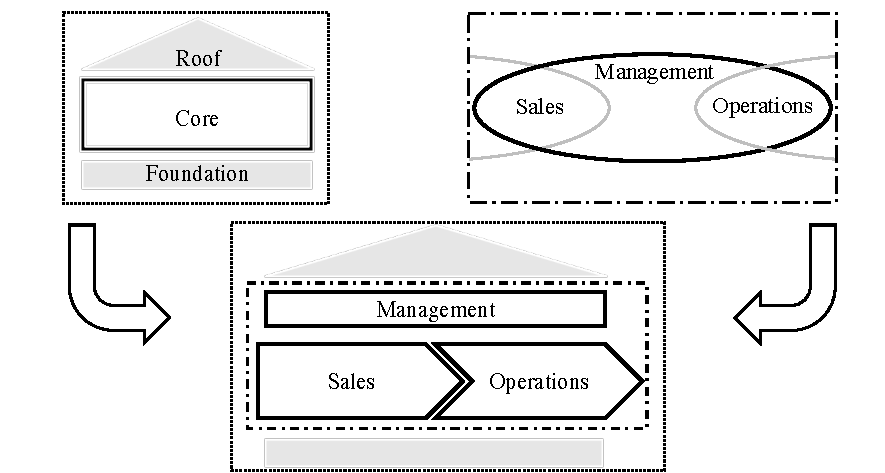
\includegraphics[width=.8\textwidth]{figures/frameworkdesign.pdf}}
	\end{figure} 
	
	
	The value chain can be represented by the exclusive use of chevrons that are linked together or it can have one starting element, which is a pentagon. This element is \textit{closed} to the left side in contrast to the \textit{open} chevrons. Porter uses the \textit{closed} variant, where the widened interface to the left side is emphasized. As the left side of the framework represents the client side, the strong link to the outsourcing partner shall be highlighted \wrt the customer-facing right hand side. Here, the interface to the customer shall be pointed for the following reasons. First, the interaction with a customer is intended to be independent of communication channel, so that the idea of omni-channel is conveyed (and with it the \textit{one face to the customer}-paradigm). Second, the customer-centric idea is communicated with this representation, as all actions towards him (the complete height of the chain) is pinpointed towards one customer. The process structure of three elements consequently locates sales processes on the left and starting part of the value chain and connects the operations processes with it, so that the client and customer side is represented. The value chain is deliberately wider than the house to make its function as an interface to the adjacent markets clear. The 
	
	The management processes are located above the value chain and spans the complete width of the house. While it is part of the core, it does not have a \acrshort{VACD} representation, as it has little contact with the the client or customer. However, it influences the complete part of business and is a indispensable part of the \acrshort{BPO} provider business, hence it must be part of the core instead of the roof. Sales processes benefit from the product and portfolio management, while workforce- and agent-related processes are scoped towards service delivery and with it operations. Reason for locating it at the top of the \acrshort{VACD} is that these processes include tactical to strategical aspects, that influence the underlying processes in the framework's core. 
	
	\subsubsection{Framework details}
	
	Locating the identified processes on the framework needs to be done carefully, as their position and shape is important for the viewer's perception. The three areas of the framework's core narrow down positioning alternatives. Their size and shape is equal, to emphasize their main process feature. Customer facing processes vary slightly. Support and Coordination processes have a smaller boxes, font size and slimmer boarders to limit their attention. \Fig \ref{fig:framework} shows the framework.
	
		\begin{figure}[caption={Framework}, label={fig:framework}]
		{	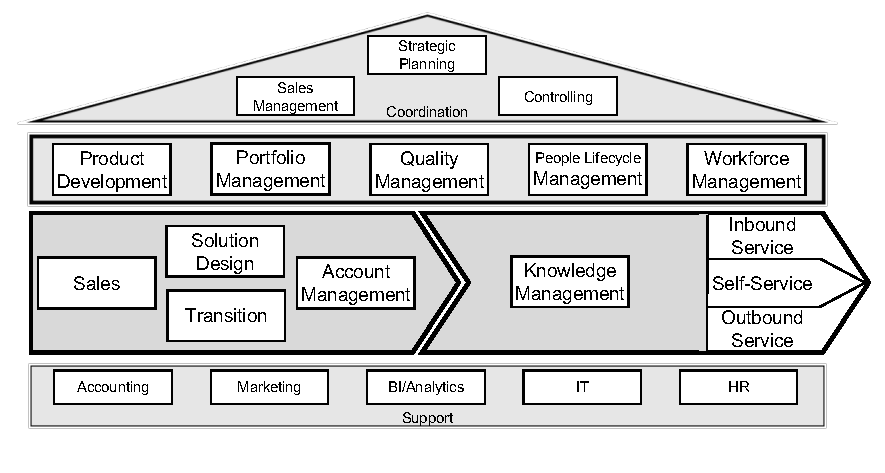
\includegraphics[width=.9\textwidth]{figures/framework.pdf}}
	\end{figure} 
	
	
	 Starting with sales-related processes, the main processes Sales, Solution Design, Implementation and Account Management have to be placed on the framework. As explained in \ref{sec:procstr}, they follow a life cycle, so that \textit{Sales} leads to \textit{Solution Design} and \textit{Implementation}, while existing clients relationships are cared in account management. This leads to a positioning of Sales as the leftmost and \textit{Account Management} as the rightmost process within the sales area. Implementation and Solution Design are processes that take between the previous ones. They are both part of the setup of a business and are hence located next to each other. 
	 
	 Operations processes have the peaked customer interface as starting point for locating processes. These are split into \textit{inbound}, \textit{outbound} and \textit{self-service} as customer facing processes, that are accompanied by\textit{ knowledge management} as an process that takes place without knowledge of the customer. Consequently, knowledge management is located towards the center of the framework and less directed to the customer. The other three processes share their direct customer contact and are therefore in the right part of the chevron. To emphasize their role as the interface to the customer, their representation is adjusted to link to the customer. Furthermore, they are also located on the same height in the flow of the chain to highlight that these are alternatives of contact. By making no distinction of channels on framework level, their equality of treatment is represented. Inbound is written on top, as it is the most important process by volume in among the three, when one sets focus on customer service.
	 
	 The four management processes are located next to each other in their area on top of the \acrshort{VACD}. The product and portfolio processes have higher connection to the client side, as these service products are sold to  clients. The \textit{product development} process has a stronger external relation, as new products should meet unsatisfied demands from the market. \textit{Portfolio management} on the other hand is an intra-organizational process that sets its focus on the provider. The other two processes, namely \textit{People Lifecycle Management} and \textit{Workforce Management} impact \acrshort{CSR}s. Their positioning can be reasoned through an higher impact of workforce management on the service delivering activities through schedules, plans and forecasts of customer demand. People Lifecycle Management on the other hand is again oriented towards the provider organization, because the management of human resources for service delivery is of direct interest for the provider, but not to the customer.
	 
	 Support and coordination processes are not further specified in this thesis. Their elements are inspired by general processes of companies that play a role in \acrshort{BPO}. Processes like accounting or marketing are obvious to fulfill financial regulations and position the provider on the market, respectively. \acrfull{BI} / Analytics captures the process of supporting the business through data-driven insights apart from implemented solutions, as well as to provide decision-support for management on a tactical or strategic level. The latter emphasizes especially the  \acrshort{BI} aspect and would also make a positioning in the roof considerable. However, analytics was added to this process as no clear border between the two can be defined in the literature  \citep{mertens}. \citep{Chen:2012:BIA} suggest the term \acrshort{BI} \& Analytics. Interpretation of the two notions will vary in an application, as it depends on the understanding in the target organization. IT supports the business through operation of systems (for instance in accounting, HR or for decision-support in management). HR manages people in the provider organization and is different from People Lifecycle Management, as it focuses on \acrshort{CSR}s, not personnel management in general. Sales Management as a coordination process is subject to planning of client businesses and verticals. It is located on the left side of the roof to move it closer to the sales processes. Strategic Planning guides the provider organization as a whole with a long-term perspective. It is located highest in the roof to emphasize its importance for the strategic management of the organization. Controlling completes the coordinating processes by supplying the management with information and overseeing the client businesses. 
	 	 
	 \subsubsection{Addressing  the design goals}
	 
	 	 	\begin{table}[caption={Design Goals}, label={tab:desobj}]
	 	\centering
	 	\begin{tabular}{l p{13.3cm}}
	 		
	 		\textbf{No. }&\textbf{ Design Goal}
	 		\\ \hline
	 		\textbf{1 }                        & The framework has to visualize the business of BPO providers.                                     \\ \hline
	 		\textbf{2}                         & The framework has distinguish business processes from other process types.                                                                                                                   \\ \hline
	 		\textbf{3 }                        & The framework has to cover the CRM-orientation in service provision. \\ \hline
	 		\textbf{4}                         & The framework has to be easily processable by viewers without further explanation.                                                              
	 		
	 	\end{tabular}
	 \end{table}
 
	 
	 With the proposed framework shown in \Fig \ref{fig:framework}, the four design goals are achieved. Its fundamental structure with the \acrshort{VACD} shows encapsulates the BPO business and by exchange of the right chevron, one can apply the model to other domains than \acrshort{CRM}. The relevance of business processes is highlighted through use of the house reference design. The right chevron is suited to represent service delivery in  \acrshort{CRM} through focus on customer contact, while abstracting from explicit processes for offered services (products). These are contained in the product development, solution design and portfolio management process without specifying of measures. Naming these would conflict with the intent of a reference model, as these will be different for companies in the domain. A minimalistic two dimensional representation without additional distracting features such as color or varying fonts supports understanding of the framework. The different shapes are limited and the use of rectangles is preferred. Other elements, like the \acrshort{VACD}, are associated by the viewer and naturally convey the flow of the framework: the outsourcing client's \acrshort{CRM} is given to the provider, who then adds the value to the chain and sends it to the customer. It is noted that application of the reference model results in differences in content, but also in design (to conform to corporate design for instance). However, an empirical evaluation of this framework design was not conducted so statements about viewer's opinions are derived from design choices of the author. \todo{rephrase}
	 
	 The following dives into the process models below the framework. The icebricks language is used to meet solution objective 4 and hence the underlying structure below the main processes on the framework is composed of detail processes, which in turn have process building block underneath. 
	 
	 
	 %%%%%%%%%%
	 \section{Customer Processes}
	 \todo{service delivery taxonomy from fitzsimmons}
	 
	 This section describes the Inbound, Outbound, Self-Service and Knowledge Management process. They describe the processing of transactions in the outsourcing contract and are driven by the target domain (\acrshort{CRM}). 
	 
	 There are several constructs by means of data, that encompass all means of contact to the outsourcing provider. First, every contact involves a customer that is asking for something or more generally put has a lack of information that should be addressed. This lack is possibly related to a product\footnote{Product here encompasses everything that is provided by the client to the market, \ie, services as well.} of the client (be it an actual purchase or solely the consideration), which is denoted as a transaction. Transactions also cover touch points like past customer service contacts or other events between the customer and the company. Together, these product-related and touch point-related transactions are determinants for forming a complete view of the customer. Transactions have a hierarchy, so that one transaction may have to a superior transaction. 
	 
	 Here, it is assumed that every transaction is related to a customer. Even if it is a new customer, the act of contacting implies a previous touch point with the company. It is noted that this transaction might be not known to the company. A customer can have multiple transactions. The contact happens as an inbound (customer contacts company), outbound (company contacts customer) or self-service (customer reaches company without involvement of a \acrshort{CSR} ). 
	 
	 Knowledge bases accessible by the outsourcing provider contain knowledge that is able to address the customer's issue that is reason for contact. As these issues are classifiable, structuring them leads to business cases that describe the solution to a known customer problem. Examples can the cancellation of a booking, the termination of a contract or change of address. This listing reveals that business cases are very dependent on the business of the client and hence are not a valid criterion for structuring customer contacts in a reference model. Not every customer contact needs to relate to a case. The \acrshort{ERM} in \Fig \ref{fig:contacterm} shows the described circumstances around the contact. It also reasons the structuring of the knowledge management process. 
	 
	 \begin{figure}[caption={\acrshort{ERM} of customer-facing services}, label={fig:contacterm}]
	 	{	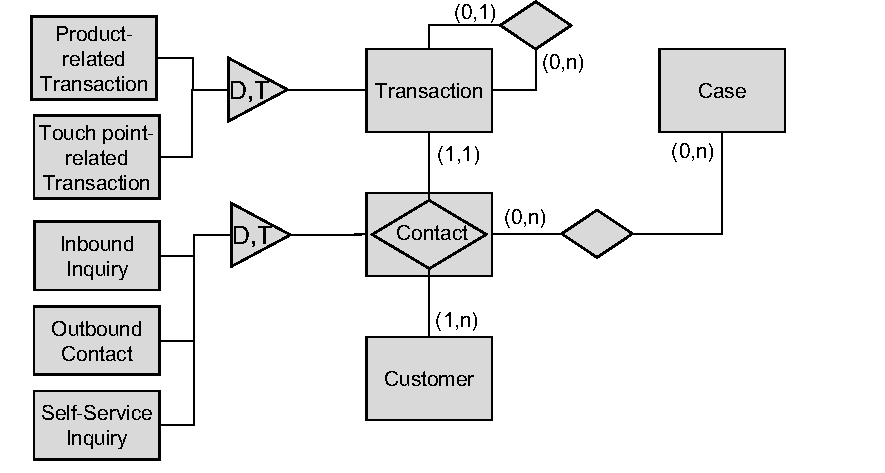
\includegraphics[width=.8\textwidth]{figures/contacterm.pdf}}
	 \end{figure} 
	 
	 
	 This analysis is necessary due to the complex and highly variable processes in Customer Service. Process Identification for Customer Service in the field of the After Sales Service as a Basis for “Lean After Sales Service”
	 im hippner buch it automation chapter für self service!
	 %%%%%%%%%%
	 Self Service: Servitization paper 1988!
	 
	 hippner:692 muss nicht nur inbound sein, outbound geht auch
	 
	 \subsection{Inbound}
	 The associated object to this process in the \textit{inquiry}\footnote{inquiry is American English; enquiry is British English.}. It is preferred over \textit{request} as it emphasizes an investigation in an issue over the politeness during asking. It is defined as an act of asking for information \citep{oxfordenquiry, oxfordrequest}. In this case, it is the customer who is lacking information in some regard and contacts the company. A \acrshort{CSR} of the outsourcing provider attends to the matter. 
	 
	 Reflections on the structure of the process become especially important in case of an omni-channel environment. There are multiple contact channels, asynchronous and synchronous communication and generic reasons that lead to the inquiry. Rationale behind omni-channel process modeling must be to keep the structure channel independent as long as possible to enable alignment. To capture the peculiarities of the channels, the concept of variants is used on the lowest level to distinguish between mail, voice, direct messenger and social channels. Reasons for this split is that other discussed channels (Video, Website, App) can be included in others by means of a process view (video to voice) or are not a contact channel by means of inbound customer service. The website and app are gateways to other channels (direct messenger) or to self-service, but do not offer direct engagement with a \acrshort{CSR}. Variants can be added, so that other channels can be easily added to the model. While there are similarities between (a)synchronous channels, using these as variants forecloses capturing of channel idiosyncrasies, because the underlying process building blocks would be the same for a variant. 
	 
	 The detail processes are structured so that their steps apply to all channels. This structuring was found to be applicable among the participants in the process modeling workshop and is shown in \Fig \ref{fig:inbproc}. First, the detail processes are described without going into details of their channel-variants. 
	 
	 \begin{figure}[caption={Inbound service process}, label={fig:inbproc}]
	 	\begin{subfigure}[b]{.45\textwidth}
	 		\begin{center}
	 			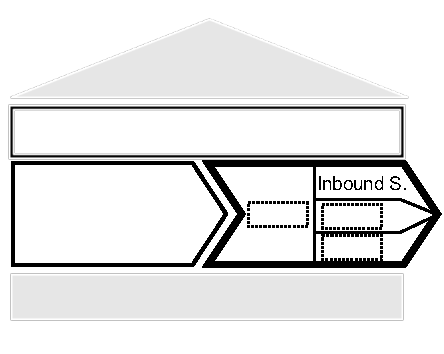
\includegraphics{figures/processes/inbound.pdf}
	 		\end{center}
	 	\end{subfigure}
	 	\begin{subfigure}[b]{.45\textwidth}
	 		\begin{center}
	 			\begin{tikzpicture}
	 			[node distance=.5cm, start chain=going below,font=\sffamily]
	 			\node[punktchain, rounded corners=0pt, join=by {-}] (eins)      {route inquiry};
	 			\node[punktchain, rounded corners=0pt, join=by {-}] (zwei) {preprocess inquiry};
	 			\node[punktchain, rounded corners=0pt, join=by {-}, ] (drei) {classify inquiry};
	 			\node[punktchain, rounded corners=0pt, join=by {-}, ] (vier) {process inquiry};
	 			\node[punktchain,rounded corners=0pt,  join=by {-}, ] (fuenf) {review inquiry};
	 			\end{tikzpicture}
	 		\end{center}
	 	\end{subfigure}
	 	
	 \end{figure}
	 
	 First, an inbound inquiry reaches is initiated by a customer and the connection with the receiving end is established. Before an interaction starts, the inquiry needs to be guided to a \acrshort{CSR}, which is known as routing in telecommunications. During this \textit{routing} process, information from the caller is processed, so that part of his needs can be inferred before the employee starts the conversation and time (and money) is consumed. On the other hand, time that the customer spends in the system before the conversation is not consuming scarce resources from the provider, so the pre-extraction of information usable to address his problem is desirable. At the end of routing, a \acrshort{CSR} is found that starts the conversation with the customer. In the \textit{preprocessing} step, the \acrshort{CSR} takes on the inquiry and consumes the information that is available from the routing, as well as transmitted by the customer. After this familiarization the \acrshort{CSR} can \textit{classify} the \textit{inquiry}, so that he knows how to map the individual inquiry of the customer to a case (if existent). The \textit{process inquiry} detail process engages the inquiry and ideally solves the problem. The last step involves a \textit{review} and closes the interaction. It updates data related to the communication and stores it in the knowledge base. As every detail process in \Fig \ref{fig:inbproc} has four variants, these are shown one by one in the following. 
	 
	 \subsubsection{Route Inquiry}
	 
	 Going into the specifics of the route inquiry detail process, \Fig \ref{fig:inbound:route} shows the four variants comprised of process building blocks. One can observe similarities 
	 across all variants, that especially in the beginning and end. During this step, no \acrshort{CSR} is actively involved.
	 \\
	 
	 \begin{figure}[caption={Route inquiry detail process}, label={fig:inbound:route}]
	 	
	 	\begin{subfigure}[b]{.45\textwidth}
	 		\centering
	 		\begin{tikzpicture}
	 		[node distance=.5cm,
	 		start chain=going below,font=\sffamily]
	 		
	 		\node[punktchain, join=by {-}] (eins)      {determine language};
	 		\node[punktchain, join=by {-}] (zwei) {analyze inquiry};
	 		\node[punktchain, join=by {-}, ] (drei) {priorize inquiry};
	 		\node[punktchain, join=by {-}, ] (vier) {select CSR};
	 		\node[punktchain, join=by {-}, ] (fuenf) {route inquiry};
	 		\node[punktchain, draw=white] (sechs) { };
	 		
	 		\end{tikzpicture}
	 		
	 		\caption{Mail variant}\label{fig:inbound:route:mail}
	 	\end{subfigure}
	 	\begin{subfigure}[b]{.45\textwidth}
	 		\centering	
	 		\begin{tikzpicture}
	 		[node distance=.5cm,
	 		start chain=going below,font=\sffamily]
	 		
	 		\node[punktchain, join=by {-}] (eins)      {determine language};
	 		\node[punktchain, join=by {-}] (zwei) {analyze inquiry};
	 		\node[punktchain, join=by {-}, ] (drei) {analyze environment};
	 		\node[punktchain, join=by {-}, ] (vier) {priorize inquiry};
	 		\node[punktchain, join=by {-}, ] (fuenf) {select CSR};
	 		\node[punktchain, join=by {-}, ] (sechs) {route inquiry};
	 		
	 		\end{tikzpicture}
	 		\caption{Social variant}\label{fig:inbound:route:social}
	 	\end{subfigure}
	 	\begin{subfigure}[b]{.45\textwidth}
	 		\centering	
	 		\begin{tikzpicture}
	 		[node distance=.5cm,
	 		start chain=going below,font=\sffamily]
	 		\node[punktchain, draw=white] (null) { };
	 		\node[punktchain] (eins)      {determine language};
	 		\node[punktchain, join=by {-}] (zwei) {collect IVR data};
	 		\node[punktchain, join=by {-}, ] (drei) {select CSR};
	 		\node[punktchain, join=by {-}, ] (vier) {route inquiry};
	 		
	 		\end{tikzpicture}
	 		\caption{Voice variant}\label{fig:inbound:route:voice}
	 	\end{subfigure}
	 	\begin{subfigure}[b]{.45\textwidth}
	 		\centering	
	 		\begin{tikzpicture}
	 		[node distance=.5cm,
	 		start chain=going below,font=\sffamily]
	 		\node[punktchain, draw=white] (null) { };
	 		\node[punktchain] (eins)      {determine language};
	 		\node[punktchain, join=by {-}] (zwei) {analzye inquiry};
	 		\node[punktchain, join=by {-}, ] (drei) {select CSR};
	 		\node[punktchain, join=by {-}, ] (vier) {route inquiry};
	 		
	 		\end{tikzpicture}
	 		\caption{Direct Messenger variant}\label{fig:inbound:route:dm}
	 	\end{subfigure}
	 \end{figure}
	 
	 A common Language is a requirement for communication and needs to be known to understand the content of the inquiry. While this is required across channels, differences arise in the following step: All variants except voice can analyze the inquiry. This analysis uses available information from the inquiry, \ie its content or channel-specific data to identify the customer and infer the customer's need. In voice the inquiry itself is not existent at this point, as the customer has not expressed it verbally. However, \acrfull{IVR} technology helps to extract information from the customer without active involvement of a \acrshort{CSR} and is a typical technology in contact centers \citep{Thomas:2009}. The distinction between voice and the other variants is reasoned by the fact that the other inquiries are text-based and therefore analyzable by common means, which is not the case for voice. As \acrshort{IVR} is a standard in customer service, the naming of a explicit technology does not create conflicts in terms of universal applicability. The amount of information processed by it varies. Simple systems might just record input from the customer typed in via the phone keypad(\textit{if you have  a question regarding X, please press 2}), while sophisticated systems do natural language processing.
	 
	 The social variant includes an \textit{analyze environment} building block, which emphasizes the importance of the network's context in social media. The verb \textit{analyze} is again used to state automatism in this step. 
	 
	 Asynchronous channels (\ie, mail, social) have a \textit{priorize inquiry} step, that work around the \acrshort{FCFS} processing of inquiries. This step is not seen for synchronous channels, as the customer actively waits for a \acrshort{CSR} to take care of his inquiry. However, as the \textit{select  \acrshort{CSR}} step takes into account several aspects, it is not said that \acrshort{FCFS} applies to synchronous channels. The selection of the  \acrshort{CSR} depends on the requirements of the inquiry (\ie, language and to that point known content of the inquiry). Means to narrow down the variety content-wise is the availability of different contact channel instances. For example, there could be a dedicated mail address for reservations and another one for bookings. The fit of inquiry requirements to agent skills is known as skill-based routing. \acrshort{CSR}s can be clustered in agent groups that are the right contact person for the inquiry, so that additional rerouting is avoided. The last process building block models the actual routing of the inquiry, as now the receiving  \acrshort{CSR} is known. This can be done with an \acrfull{ACD} technology\footnote{Despite its naming, the technology is able to route calls of other channels \citep{ccn2016} } which is able to take available client and agent information into account.
	 
	 
	 \subsubsection{Preprocess Inquiry}
	 
	 This detail process, shown in \Fig \ref{fig:inbound:prepr}, begins with a \acrshort{CSR} entering the process, that consumes the available information of the inquiry. This is not possible on the voice channel. There, the agent needs to open the conversation first, followed by the listening to the customer. Then he obtains understanding of the problem and can checks whether the data form the \acrshort{IVR} is correct. The other channels, analogous to the route inquiry detail process, \textit{check analytical results} so that there is consensus of manually read inquiry content and analytically derived aspects.
	 
	 In the same way, the social variant includes a manual verification of the environment in the network. As elements can be skipped if not applicable (\ie no analytical system in place to check the environment in the social network), this building block may be interpreted as a first check of the environmental situation. Contextual factors (related posts with the same issue) on the facebook wall for instance may require a different approach towards the inquiry to ensure the appropriate reaction of the company in public.   
	 
	 The synchronous channels, \ie, \Fig \ref{fig:inbound:prepr:voice}, \ref{fig:inbound:prepr:dm} show time-logic differences. While the voice channel needs to open the conversation to know about the inquiry, a \acrshort{CSR} in a direct messenger communication is able to do the preprocessing step beforehand and opens the conversation to the customer at the end. 
	 
	 \begin{figure}[caption={Preprocess inquiry detail process}, label={fig:inbound:prepr}]
	 	
	 	\begin{subfigure}[b]{.45\textwidth}
	 		\centering
	 		\begin{tikzpicture}
	 		[node distance=.5cm,
	 		start chain=going below,font=\sffamily]
	 		
	 		\node[punktchain, join=by {-}] (eins)      {read inquiry};
	 		\node[punktchain, join=by {-}] (zwei) {check analytical results};
	 		\node[punktchain,  draw=white,text=white] (sechs) {  verify environment};
	 		
	 		\end{tikzpicture}
	 		
	 		\caption{Mail variant}\label{fig:inbound:prepr:mail}
	 	\end{subfigure}
	 	\begin{subfigure}[b]{.45\textwidth}
	 		\centering	
	 		\begin{tikzpicture}
	 		[node distance=.5cm,
	 		start chain=going below,font=\sffamily]
	 		
	 		\node[punktchain, join=by {-}] (eins)      {read inquiry};
	 		\node[punktchain, join=by {-}] (zwei) {check analytical results};
	 		\node[punktchain, join=by {-}, ] (drei) {check environment};
	 		
	 		
	 		\end{tikzpicture}
	 		\caption{Social variant}\label{fig:inbound:prepr:social}
	 	\end{subfigure}
	 	\begin{subfigure}[b]{.45\textwidth}
	 		\centering	
	 		\begin{tikzpicture}
	 		[node distance=.5cm,
	 		start chain=going below,font=\sffamily]
	 		\node[punktchain, draw=white] (null) { };
	 		\node[punktchain] (eins)      {open conversation};
	 		\node[punktchain, join=by {-}] (zwei) {listen to inquiry};
	 		\node[punktchain, join=by {-}, ] (drei) {check IVR data};
	 		
	 		
	 		\end{tikzpicture}
	 		\caption{Voice variant}\label{fig:inbound:prepr:voice}
	 	\end{subfigure}
	 	\begin{subfigure}[b]{.45\textwidth}
	 		\centering	
	 		\begin{tikzpicture}
	 		[node distance=.5cm,
	 		start chain=going below,font=\sffamily]
	 		\node[punktchain, draw=white] (null) { };
	 		\node[punktchain] (zwei) {read inquiry};
	 		\node[punktchain, join=by {-}, ] (drei) {check analytical results};
	 		\node[punktchain, join=by {-}, ] (vier) {open conversation};
	 		
	 		\end{tikzpicture}
	 		\caption{Direct Messenger variant}\label{fig:inbound:prepr:dm}
	 	\end{subfigure}
	 \end{figure}
	 
	 
	 \subsubsection{Classify Inquiry}
	 
	 \Fig \ref{fig:inbound:class} shows the four variants for the third detail process of the inbound process. One can see that there is no difference seen between asynchronous (top row) and synchronous (lower row), so it is possible to shrink the representation down to two variants or even one variant, as the \textit{request missing information} building block can be skipped in the icebricks language if not applicable. For the sake of consistency across all detail processes, the four variant split is preserved.
	 
	 \begin{figure}[caption={Classify inquiry detail process}, label={fig:inbound:class}]
	 	
	 	
	 	\begin{subfigure}[b]{.45\textwidth}
	 		\centering
	 		\begin{tikzpicture}
	 		[node distance=.5cm,
	 		start chain=going below,font=\sffamily]
	 		
	 		\node[punktchain, join=by {-}] (eins)      {combine available information};
	 		\node[punktchain, join=by {-}] (zwei) {correct analytical mistakes};
	 		\node[punktchain, join=by {-}] (drei) {classify inquiry};
	 		
	 		
	 		\end{tikzpicture}
	 		
	 		\caption{Mail variant}\label{fig:inbound:class:mail}
	 	\end{subfigure}
	 	\begin{subfigure}[b]{.45\textwidth}
	 		\centering	
	 		\begin{tikzpicture}
	 		[node distance=.5cm,
	 		start chain=going below,font=\sffamily]
	 		
	 		\node[punktchain, join=by {-}] (eins)      {combine available information};
	 		\node[punktchain, join=by {-}] (zwei) {correct analytical mistakes};
	 		\node[punktchain, join=by {-}] (drei) {classify inquiry};
	 		
	 		\end{tikzpicture}
	 		\caption{Social variant}\label{fig:inbound:class:social}
	 	\end{subfigure}
	 	\begin{subfigure}[b]{.45\textwidth}
	 		\centering	
	 		\begin{tikzpicture}
	 		[node distance=.5cm,
	 		start chain=going below,font=\sffamily]
	 		\node[punktchain, draw=white] (null) { };
	 		\node[punktchain] (eins)      {combine available information};
	 		\node[punktchain, join=by {-}] (zwei) {correct analytical mistakes};
	 		\node[punktchain, join=by {-}] (drei) {request missing information};
	 		\node[punktchain, join=by {-}] (vier) {classify inquiry};
	 		
	 		
	 		\end{tikzpicture}
	 		\caption{Voice variant}\label{fig:inbound:class:voice}
	 	\end{subfigure}
	 	\begin{subfigure}[b]{.45\textwidth}
	 		\centering	
	 		\begin{tikzpicture}
	 		[node distance=.5cm,
	 		start chain=going below,font=\sffamily]
	 		\node[punktchain, draw=white] (null) { };
	 		\node[punktchain] (eins)      {combine available information};
	 		\node[punktchain, join=by {-}] (zwei) {correct analytical mistakes};
	 		\node[punktchain, join=by {-}] (drei) {request missing information};
	 		\node[punktchain, join=by {-}] (vier) {classify inquiry};
	 		
	 		\end{tikzpicture}
	 		\caption{Direct Messenger variant}\label{fig:inbound:class:dm}
	 	\end{subfigure}
	 \end{figure}
	 
	 First, the available information of the inquiry and the analytical support from the two previous detail processes is combined to form one understanding of the inquiry for the \acrshort{CSR}. Next, mistakes of the analytical support are corrected, so that the system gets feedback and may improve in future.
	 
	 Third, the \textit{ classify inquiry} building block connects the inquiry (up to here seen as an instantiation of an unknown case) to a class. This class is a known construct in the mind of the \acrfull{CSR} and ideally described in a knowledge base as a case. An example for this split is an inquiry by a customer a, that expresses his wish to swap his ticket of x on day y to day z. The \acrshort{CSR} can classify this inquiry as class \textit{change of booking}. With this link being established, the problem is understood by the  \acrshort{CSR} and inquiry processing can be commenced. 
	 
	 Synchronous channels contain a \textit{request additional information} building block, that enables the \acrshort{CSR} to get additional information from the customer needed prior to classification(a booking number is required for a change of booking and not known). This is put before classification, so that a class can have requirements that need to be fulfilled before assignment. By this logic, the \acrshort{CSR} needs to have a guess about the customer's need, so that the right information is requested.  
	 
	 This classification of the inquiry, \ie, the mapping of the customers individually expressed needs to a modeled case on company/provider-side is seen as the essential task of the \acrshort{CSR} here. If the case was correctly modeled and identified, in theory its process would be adequately represented by \acrshort{IS} and no human involvement from the customer service side would be necessary. 
	 
	 \subsubsection{Process Inquiry}
	 
	 The process inquiry detail process is shown in \Fig \ref{fig:inbound:proc}. It represents the addressing of the customer need, that was previously defined and classified. Similarities among all variants are the starting building block \textit{query knowledge base}. This models the \acrshort{CSR}'s lookup of information related to the case at hand, either to give the requested information to the customer or to look up the process to solve the customer's issue.  
	 
	 Asynchronous channels, \Fig \ref{fig:inbound:proc:mail}, \ref{fig:inbound:proc:social}, contain a \textit{draft response} building block. Draft is used to enable the possibility of a following review step. Response on the other hand represents the asynchronous property of the communication. The response to the inquiry does not necessarily solve the customer's problem, as no conversation is included that verifies the correct understanding of the problem. Synchronous channels are assumed to solve the inquiry within the bounds of possibility. 
	 
	 The models on the right side of \Fig \ref{fig:inbound:proc} both contain a \textit{check-privacy guidelines} and \textit{request channel switch} building block. As direct messengers or social networks are often platforms, operated by other parties that may have a different understanding of data privacy, certain business cases cannot be processed on these channels. Hence, a channel switch becomes necessary and ends the process. 
	 
	 The voice channel additionally includes an identification segment, that represents the \acrshort{CSR}s ability to verify the customer's identity during the conversation. This does not represent the identification of the customer to an entry in the \acrshort{CRM} database, but a legally binding statement, that may be required for certain business cases. Video communication is a means to achieve the certainty of identity for the \acrshort{CSR}.
	 A channel like mail lacks the ability to identify a customer, as everyone with access to the customer's account can send on his behalf. This represents knowledge at the time of writing based on current practice. In future, a legally binding identification over different channels might be possible, for example via social media profile.
	 
	 
	 \begin{figure}[caption={Process inquiry detail process}, label={fig:inbound:proc}]
	 	
	 	\begin{subfigure}[b]{.45\textwidth}
	 		\centering
	 		\begin{tikzpicture}
	 		[node distance=.5cm,
	 		start chain=going below,font=\sffamily]
	 		
	 		\node[punktchain, join=by {-}] (eins)      {query knowledge base};
	 		\node[punktchain, join=by {-}] (zwei) {draft response};
	 		\node[punktchain, text=white,draw=white] (drei) {request missing information};
	 		\node[punktchain, text=white,draw=white] (vier) {classify inquiry};
	 		
	 		
	 		\end{tikzpicture}
	 		
	 		\caption{Mail variant}\label{fig:inbound:proc:mail}
	 	\end{subfigure}
	 	\begin{subfigure}[b]{.45\textwidth}
	 		\centering	
	 		\begin{tikzpicture}
	 		[node distance=.5cm,
	 		start chain=going below,font=\sffamily]
	 		
	 		\node[punktchain, join=by {-}] (eins)      {query knowledge base};
	 		\node[punktchain, join=by {-}] (zwei) {check privacy guidelines};
	 		\node[punktchain, join=by {-}] (drei) {request channel switch};
	 		\node[punktchain, join=by {-}] (vier) {draft response};
	 		
	 		\end{tikzpicture}
	 		\caption{Social variant}\label{fig:inbound:proc:social}
	 	\end{subfigure}
	 	\begin{subfigure}[b]{.45\textwidth}
	 		\centering	
	 		\begin{tikzpicture}
	 		[node distance=.5cm,
	 		start chain=going below,font=\sffamily]
	 		\node[punktchain, draw=white] (null) { };
	 		\node[punktchain] (eins)      {query knowledge base};
	 		\node[punktchain, join=by {-}] (zwei) {request identification};
	 		\node[punktchain, join=by {-}] (drei) {identify customer};
	 		\node[punktchain, join=by {-}] (vier) {solve inquiry};
	 		
	 		
	 		\end{tikzpicture}
	 		\caption{Voice variant}\label{fig:inbound:proc:voice}
	 	\end{subfigure}
	 	\begin{subfigure}[b]{.45\textwidth}
	 		\centering	
	 		\begin{tikzpicture}
	 		[node distance=.5cm,
	 		start chain=going below,font=\sffamily]
	 		\node[punktchain, draw=white] (null) { };
	 		\node[punktchain] (eins)      {query knowledge base};
	 		\node[punktchain, join=by {-}] (zwei) {check privacy guidelines};
	 		\node[punktchain, join=by {-}] (drei) {request channel switch};
	 		\node[punktchain, join=by {-}] (vier) {solve inquiry};
	 		
	 		\end{tikzpicture}
	 		\caption{Direct Messenger variant}\label{fig:inbound:proc:dm}
	 	\end{subfigure}
	 \end{figure}
	 
	 
	 \subsubsection{Review Inquiry}
	 \label{inb:review}
	 Review inquiry is the last detail process within the inbound process. Its four variants can be inspected in \Fig \ref{fig:inbound:revw}. Two meanings of the notion of review in the Oxford Dictionary \citep{oxfordreview} fit to explain the different variants. First, a review is a \enquote{formal assessment of something with the intention of instituting change if necessary}. This definition fits to describe building blocks in asynchronous channels mail and social. A \acrshort{CSR} might need to send a response to a supervisor for checking. The supervisor can change parts or approve it directly (called \textit{finalize} here). In social networks, the environment should be checked again, as it could have changed since compilation of the draft. Also, the submission of the response is called \textit{posting} to emphasize differences of public posting to private \textit{sending} of mails.
	 
	 Synchronous channels (\cf \Fig \ref{fig:inbound:revw:voice}, \ref{fig:inbound:revw:dm}) show the same components, that are again not aggregated into one variant for consistency reasons. As they solve the inquiry during the synchronous conversation, no review according to the given definition is possible. However, second meaning of the term review explains the purpose of this step: \enquote{A report on or evaluation of a subject or past events}. 
	 
	 This justifies the last two process building blocks of all three variants, namely \textit{update customer data} and \textit{update inquiry}. As the interaction is completed at this point (\viz the response is sent, posted and the synchronous conversation is closed), information from the customer contact is to be stored. On the one hand, the customer contact, seen as a touch point and therefore a transaction, is connected to the customer in the \acrshort{CRM} data base. Additional data that might be revealed during the contact can also be stored to enrich the profile by the \acrshort{CSR}. Furthermore, the inquiry itself can be updated to keep track of the customer's issue if not solved entirely. Ticket systems are a concept to model this matter. The system itself  keeps track of handling times and other measures of the inquiry, so that data for reporting is generated. 
	 
	 
	 \begin{figure}[caption={Review inquiry detail process}, label={fig:inbound:revw}]
	 	
	 	\begin{subfigure}[b]{.45\textwidth}
	 		\centering
	 		\begin{tikzpicture}
	 		[node distance=.5cm,
	 		start chain=going below,font=\sffamily]
	 		
	 		\node[punktchain, join=by {-}] (eins)      {review response};
	 		\node[punktchain, join=by {-}] (zwei) {finalize response};
	 		\node[punktchain, join=by {-}] (drei) {send response};
	 		\node[punktchain, join=by {-}] (vier) {update customer data};
	 		\node[punktchain, join=by {-}] (fuenf) {update inquiry};
	 		\node[punktchain, draw=white,text=white] (sechs) {verify environment};
	 		
	 		\end{tikzpicture}
	 		
	 		\caption{Mail variant}\label{fig:inbound:revw:mail}
	 	\end{subfigure}
	 	\begin{subfigure}[b]{.45\textwidth}
	 		\centering	
	 		\begin{tikzpicture}
	 		[node distance=.5cm,
	 		start chain=going below,font=\sffamily]
	 		
	 		\node[punktchain, join=by {-}] (eins)      {review response};
	 		\node[punktchain, join=by {-}] (zwei) {verify environment};
	 		\node[punktchain, join=by {-}] (drei) {finalize response};
	 		\node[punktchain, join=by {-}] (vier) {post response};
	 		\node[punktchain, join=by {-}] (fuenf) {update customer data};
	 		\node[punktchain, join=by {-}] (sechs) {update inquiry};
	 		
	 		\end{tikzpicture}
	 		\caption{Social variant}\label{fig:inbound:revw:social}
	 	\end{subfigure}
	 	\begin{subfigure}[b]{.45\textwidth}
	 		\centering	
	 		\begin{tikzpicture}
	 		[node distance=.5cm,
	 		start chain=going below,font=\sffamily]
	 		\node[punktchain, draw=white] (null) { };
	 		\node[punktchain] (eins)      {close conversation};
	 		\node[punktchain, join=by {-}] (zwei) {update customer data};
	 		\node[punktchain, join=by {-}] (drei) {update inquiry};
	 		\end{tikzpicture}
	 		\caption{Voice variant}\label{fig:inbound:revw:voice}
	 	\end{subfigure}
	 	\begin{subfigure}[b]{.45\textwidth}
	 		\centering	
	 		\begin{tikzpicture}
	 		[node distance=.5cm,
	 		start chain=going below,font=\sffamily]
	 		\node[punktchain, draw=white] (null) { };
	 		\node[punktchain] (eins) {close conversation};
	 		\node[punktchain, join=by {-}] (zwei) {update customer data};
	 		\node[punktchain, join=by {-}] (drei) {update inquiry};
	 		
	 		\end{tikzpicture}
	 		\caption{Direct Messenger variant}\label{fig:inbound:revw:dm}
	 	\end{subfigure}
	 \end{figure}
	 
	 
	 
	 
	 
	 
	 
	 
	 \subsection{Self-Service}
	 
	 The third customer interaction process leaves inter-personal service \citep{Thomas2008self} and focuses on ways that enable the customer to be the main value-generating part in the service interaction. This is facilitated by a technological component which can relieve the customer of a varying extent of the problem. The following illustrates this continuum from a customer perspective: Simple self-services, like an \acrshort{FAQ} section offer answers to questions, which the customer has to select from a list. The customer must express the need, map it to the available information, select the appropriate answer and process its content. A more advanced self-service might be able to additionally support the customer by the expression of the need and takes care of the mapping by a textual input, which is a more natural way of communication. The textual is analyzed and algorithmically mapped to the most appropriate solution, which is then presented to the customer, who must consume its content and is hopefully satisfied. It is noted that both solutions address the customer's issue, but sophisticated \acrshort{IT} increases usability by an easier interface to the customer's issue and a computed provision of a solution. This addresses what \citep{Thomas2008self} names a minimal skill set, \viz the an increased usability decreases the minimal skill set that is required for use. 
	 
	 From literature \citep{meuter2000self, Thomas2008self, Thomas:2009}, one can identify characteristics of self-services, which need to be considered in a process. As in the model the perspective of the service provider is chosen, the process needs to hold aspects which are seen from a system perspective. The previous example features the differences between a simple and technological enhanced serf-service. In both cases, the system has to provide information, but the simple self-services required the capability to express the need in the language of the service system, while the second allowed the customer to express it more naturally. The system perspective implies that the more active the customer takes the part in the process (\ie the simpler the self-service is), the less parts of the process are carried out by the system. 
	 
	 Furthermore, a self-service can be seen as part of a another customer service process. One can think of a self-service as support for a inter-personal contact, when it provides solutions based on customer information. Examples for this are \acrshort{IVR} or generated chat messages based on customer input.
	 
	 Unlike inter-personal services, self-services cannot be structured \wrt a communication channel, as they can be part of a service within one or multiple channels, or stand-alone in a web-based setting. A process representation is chosen which models both a supporting self-service for other services and a stand-alone implementation.
	 
	 \begin{figure}[caption={Self-Service process}, label={fig:selfservice}]
	 	\begin{subfigure}[b]{.45\textwidth}
	 		\begin{center}
	 			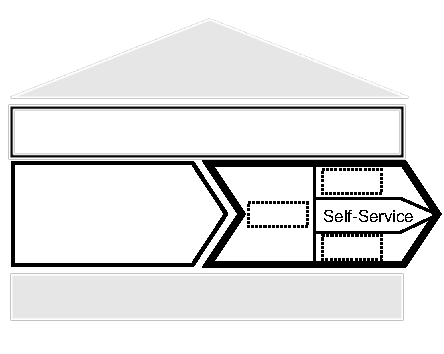
\includegraphics{figures/processes/selfservice.pdf}
	 		\end{center}
	 	\end{subfigure}
	 	\begin{subfigure}[b]{.45\textwidth}
	 		\begin{center}
	 			\begin{tikzpicture}
	 			[node distance=.5cm, start chain=going below,font=\sffamily]
	 			\node[punktchain, rounded corners = 0pt, join=by {-}] (eins)      {identify customer needs};
	 			\node[punktchain,  rounded corners = 0pt,  join=by {-}] (zwei) {process customer needs};
	 			\node[punktchain,  rounded corners = 0pt, join=by {-}, ] (drei) {present solution};
	 			\node[punktchain, rounded corners = 0pt,  join=by {-}, ] (vier) {evaluate solution};
	 			
	 			\end{tikzpicture}
	 		\end{center}
	 	\end{subfigure}
	 	
	 \end{figure}
	 
	 The process object customer need is chosen over inquiry to express the differences over inbound processing. It is noted that a customer need is an abstract construct that is used to express the customer's intention of use. However, like the inbound process self-service gets input from a customer and tries to solve the issue. But as there is no \acrshort{CSR} directly involved, there is less certainty that the system adequately addresses the \enquote{inquiry}. Due to this lack of a human counterpart on provider side, the technological interface provided by the system to the customer takes an important part in \textit{identifying customer needs}. As the capabilities of this interface vary drastically among different self-service scenarios, customer needs are chosen to emphasize the difference to inbound processing. \textit{Process customer needs} then aims at mapping the identified need to a defined solution in the knowledge base. After creation, \textit{present solution} communicates the findings to the customer. Lastly, \textit{evaluate solution} represents post-processing activities. The process is shown in \Fig \ref{fig:selfservice}.
	 
	 The building blocks of the four detail processes are summarized in \Fig \ref{fig:selfservice:detail}, as their is no further split into variants. The following description emphasizes the differences in simple and advanced self-service scenarios. 
	 
	 The building blocks of \textit{identfiy customer needs} (\Fig \ref{fig:selfservice:1}) capture external circumstances, that might be processed by the system to have more data available for inferring the customer need. Environmental factors are implicitly collected, \ie the customer does not need to state them. Request information models the input that the customer gives to the system. While the active phrasing might fit to more advanced self-service systems better than to simple \acrshort{FAQ}s, as the latter hardly asks the customer for information, the step applies to the concept of self-services: in order to narrow down the customer needs, relevant information needs to be selected by the customer (in a simple self-service system) or demanded as input for the system (in the advanced case). The verb \textit{infer} is used to describe the stochastic component of the system's attempt to understand the customer need. Again, the selection of a \acrshort{FAQ} entry by the customer might minimize the system's influence, still it conceives the selection as an information input and infers that the customer is \textit{needing} answers in this regard. An increased usability in the technological interface (arbitrary text input instead of a selection of options) also increases uncertainty in need identification, because the system has to select the fitting case by itself. 
	 
	 After the customer needs are inferred and hence available in a manner that corresponds to the data available in the knowledge base, the \textit{process customer needs} detail process (\Fig \ref{fig:selfservice:2}) receives  suitable information and creates a solution based on it. The solution represents the appropriate response to the customer's need. This can be the needed information, so that the need is completely addressed. Another option is that the self-service system can identify the need, but solving it requires personal-interaction. This expresses the limitations of service automation. 
	 
	 \textit{Present solution} (\Fig \ref{fig:selfservice:3}) conveys the result to the customer. The solution is presented by the system and is an adequate response to the customer's input. The customer's reaction is an important indicator of satisfaction and captured during the presentation. As the identification of a customer is not required for self-service use, these data needs to be stored in relation to the self-service input to further improve customer experience. The last detail process \textit{evaluate solution} (\Fig \ref{fig:selfservice:4}) can include a request for feedback (\enquote{Did this solve your problem?}) and finally all relevant information of the self-service use is stored and hence updates knowledge base. 
	 
	 \begin{figure}[caption={Self-service detail processes}, label={fig:selfservice:detail}]
	 	
	 	\begin{subfigure}[b]{.45\textwidth}
	 		\centering
	 		\begin{tikzpicture}
	 		[node distance=.5cm,
	 		start chain=going below,font=\sffamily]
	 		
	 		\node[punktchain, join=by {-}] (eins)      {analyze environment};
	 		\node[punktchain, join=by {-}] (zwei)      {request information};
	 		\node[punktchain, join=by {-}] (eins)      {infer customer needs};
	 		
	 		
	 		\end{tikzpicture}
	 		
	 		\caption{Identify customer needs}\label{fig:selfservice:1}
	 	\end{subfigure}
	 	\begin{subfigure}[b]{.45\textwidth}
	 		\centering	
	 		\begin{tikzpicture}
	 		[node distance=.5cm,
	 		start chain=going below,font=\sffamily]
	 		
	 		\node[punktchain, join=by {-}] (zwei) {query knowledge base};
	 		%	\node[punktchain, join=by {-}] (zwei) {integrate subsystem information};
	 		\node[punktchain, join=by {-}] (drei) {create solution};
	 		\node[punktchain, draw=white,text=white] (sechs) {verify environment};
	 		\end{tikzpicture}
	 		\caption{Process customer needs}\label{fig:selfservice:2}
	 	\end{subfigure}
	 	\begin{subfigure}[b]{.45\textwidth}
	 		\centering	
	 		\begin{tikzpicture}
	 		[node distance=.5cm,
	 		start chain=going below,font=\sffamily]
	 		\node[punktchain, draw=white] (null) { };
	 		\node[punktchain] (eins)      {present solution};
	 		\node[punktchain, join=by {-}] (zwei) {process customer reaction};
	 		\end{tikzpicture}
	 		\caption{Present solution}\label{fig:selfservice:3}
	 	\end{subfigure}
	 	\begin{subfigure}[b]{.45\textwidth}
	 		\centering	
	 		\begin{tikzpicture}
	 		[node distance=.5cm,
	 		start chain=going below,font=\sffamily]
	 		\node[punktchain, draw=white] (null) { };
	 		\node[punktchain] (eins) {request feedback};
	 		\node[punktchain, join=by {-}] (zwei) {update knowledge base};
	 		
	 		\end{tikzpicture}
	 		\caption{Evaluate solution}\label{fig:selfservice:4}
	 	\end{subfigure}
	 \end{figure}
	 
	 
	 
	 
	 klar definieren was ich unter sst verstehe \citep{Thomas:2009} hält auch online tech support boards, live chat sessions with customer support personal, user forums, etc. drin. also da wo der CSR noch supported. 
	 starting point \citep{Thomas:2009}.
	 %When a customer calls into the call center for technical support, it is often with the belief that they are contacting a CSR who is either an expert at solving their problem or at least more knowledgeable about their problem than the caller.
	 \citep{ccn2016} s.44
	 
	 %	To determine the most efficient, effective and mutually acceptable use of technology in service delivery, the customer's perspective needs to be known and understood.  \citep{Walker_2002}
	 
	 
	 \newpage
	 \newpage
	 
	 \subsection{Outbound Service}
	 
	 In contrast to inbound interactions that have an inquiry as central object of the process, the outreaching communications do not necessarily target a customer's issue. Its root depends on the purpose of the communication, which can be related to a previous interaction (call-back service in voice) or e-mail marketing (new offers via mail) for instance. Therefore, the general term \textit{contact} is used and defined as \enquote{a meeting, communication, or relationship with someone} \citep{oxfordcontact}. The verb refers to the communication with someone.
	 
	 Alike to inbound processing, omni-channel applicability is enabled by having a universal detail process, which has variants for each of the four contact channel categories. It is noted that outbound communication may apply differently across the channel types and dependent on implemented technology. There is the necessity of knowing the identifier of a customer within a contact channel to reach him. This identifier is the phone number in voice, mail address or a social media account. Direct messengers may be designed to enable use without individual sign-up, which excludes the ability to reach the customer. However, using direct messenger platforms such as WhatsApp enables outgoing communications, as work with identifiers. 
	 
	 \begin{figure}[caption={Outbound service process}, label={fig:outbound}]
	 	\begin{subfigure}[b]{.45\textwidth}
	 		\begin{center}
	 			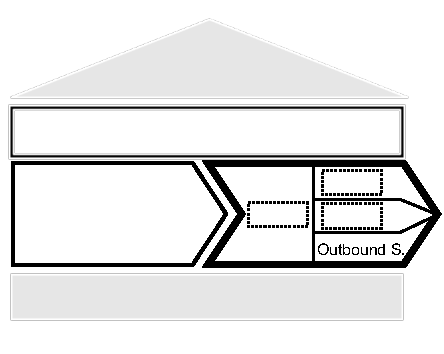
\includegraphics{figures/processes/outbound.pdf}
	 		\end{center}
	 	\end{subfigure}
	 	\begin{subfigure}[b]{.45\textwidth}
	 		\begin{center}
	 			\begin{tikzpicture}
	 			[node distance=.5cm, start chain=going below,font=\sffamily]
	 			\node[punktchain,rounded corners=0pt, join=by {-}] (eins)      {prepare contact};
	 			\node[punktchain,rounded corners=0pt, join=by {-}] (zwei) {contact customer};
	 			\node[punktchain,rounded corners=0pt, join=by {-}, ] (drei) {evaluate contact};
	 			\node[punktchain, draw=white ] (vier) { };
	 			
	 			\end{tikzpicture}
	 		\end{center}
	 	\end{subfigure}
	 	
	 \end{figure}
	 
	 
	 
	 
	 A fundamental difference the inbound and outbound process is that outbound contact is proactive and needs more initial information to act on, whereas inbound contact is more reactive \citep{DimensionData2015}. \Fig \ref{fig:outbound} shows the detail process, which is composed of three steps. As an analogy to the inbound detail process, the \textit{prepare contact} represents activities that take place prior to the activity that actually addresses the process object (route, preprocess, classify inquiry in the inbound process). The following \textit{contact customer} step expresses the active approach of the customer (contact) from the company side and can mirror the process inquiry step in the inbound process. Lastly, the \textit{evaluate contact} step contains subsequent efforts. Here the wording evaluate is chosen over review to put more focus on an assessment of the contact and less on the intention to change parts if necessary (\cf \ref{inb:review}). Furthermore, the company as contact initiator can perform a review at an earlier stage and does not need to react on a customer. 
	 
	 
	 \subsubsection{Prepare Contact}
	 
	 To actively approach a customer, there has to be a trigger or decision that lead to the initiation of the process, which is then assigned to the executing organizational unit, \ie \acrshort{CSR}. The information that captures the intention behind the contact is assumed to be stored in the knowledge base. The first step of this detail process (\Fig \ref{fig:outbound:prep}) is consequently a query to get the \acrshort{CSR} informed, which is consistent over all channel variants. Next, the aforementioned reason for contact is processed by the \acrshort{CSR} to enable the transfer of it towards the upcoming contact of the customer. 
	 
	 All channels except voice show three blocks, that also appear in the review inquiry inbound process variant (draft, review, finalize message/post). This early (optional) verification by a supervisor is possible because the communication is started by the company and the purpose is stored in the known reason for contact. Therefore, there is no processing of a customer inquiry necessary on which a response is formulated. Because of this, direct messengers can also have these component, even though it is a synchronous channel. In the voice variant, there is no review. The \acrshort{CSR} is assumed to understand the reason for contact or resolve any issues with it in the \textit{process reason for contact} step, as the scripting of a call is implausible. 
	 
	 The case of a proactive post of a company on a customer's social profile might seem less typical on platforms like facebook, but it cannot be foreclosed. In addition, it depends on the social behavior on the network that might change over time and varies across networks.  
	 
	 \begin{figure}[caption={Prepare contact detail process}, label={fig:outbound:prep}]
	 	
	 	\begin{subfigure}[b]{.45\textwidth}
	 		\centering
	 		\begin{tikzpicture}
	 		[node distance=.5cm,
	 		start chain=going below,font=\sffamily]
	 		
	 		\node[punktchain, join=by {-}] (eins)      {query knowledge base};
	 		\node[punktchain, join=by {-}] (zwei) {process reason for contact};
	 		\node[punktchain, join=by {-}] (drei) {draft message};
	 		\node[punktchain, join=by {-}] (vier) {review message};
	 		\node[punktchain, join=by {-}] (fuenf) {finalize message};
	 		
	 		\end{tikzpicture}
	 		
	 		\caption{Mail variant}\label{fig:outbound:prep:mail}
	 	\end{subfigure}
	 	\begin{subfigure}[b]{.45\textwidth}
	 		\centering	
	 		\begin{tikzpicture}
	 		[node distance=.5cm,
	 		start chain=going below,font=\sffamily]
	 		
	 		\node[punktchain, join=by {-}] (eins)      {query knowledge base};
	 		\node[punktchain, join=by {-}] (zwei) {process reason for contact};
	 		\node[punktchain, join=by {-}] (drei) {draft post};
	 		\node[punktchain, join=by {-}] (vier) {review post};
	 		\node[punktchain, join=by {-}] (fuenf) {finalize post};
	 		\end{tikzpicture}
	 		\caption{Social variant}\label{fig:outbound:prep:social}
	 	\end{subfigure}
	 	\begin{subfigure}[b]{.45\textwidth}
	 		\centering	
	 		\begin{tikzpicture}
	 		[node distance=.5cm,
	 		start chain=going below,font=\sffamily]
	 		\node[punktchain, draw=white] (null) { };
	 		\node[punktchain] (eins)      {query knowledge base};
	 		\node[punktchain, join=by {-}] (zwei) {process reason for contact};
	 		\node[punktchain, draw=white] (null) { };
	 		\node[punktchain, draw=white] (null) { };
	 		\node[punktchain, draw=white] (null) { };
	 		
	 		\end{tikzpicture}
	 		\caption{Voice variant}\label{fig:outbound:prep:voice}
	 	\end{subfigure}
	 	\begin{subfigure}[b]{.45\textwidth}
	 		\centering	
	 		\begin{tikzpicture}
	 		[node distance=.5cm,
	 		start chain=going below,font=\sffamily]
	 		\node[punktchain, draw=white] (null) { };
	 		\node[punktchain] (eins) {query knowledge base};
	 		\node[punktchain, join=by {-}] (zwei) {process reason for contact};
	 		\node[punktchain, join=by {-}] (drei) {draft message};
	 		\node[punktchain, join=by {-}] (vier) {review message};
	 		\node[punktchain, join=by {-}] (fuenf) {finalize message};
	 		
	 		\end{tikzpicture}
	 		\caption{Direct Messenger variant}\label{fig:outbound:prep:dm}
	 	\end{subfigure}
	 \end{figure}
	 
	 
	 \subsubsection{Contact Customer}
	 
	 The second step of the outbound process models the approach of the client (\Fig \ref{fig:outbound:con}) . The use of contact as a verb expresses that the customer is on the receiving end. (A)synchronous channels show a similar structure, respectively. As the message or post is already prepared, the select of the sending account and the actual transmission\footnote{Theoretically, the second block in the social variant should be named \textit{post post}. Considering writing style, the object is kept and the verb changed to send. } is left. As previously justified, the variant in social media includes a verification step of the network environment. 
	 
	 Synchronous communication establishes a \textit{conversation} with the customer on which is responded in a timely manner. It is noted that in contrast to the voice channel, a direct message does not require the customer to respond directly to the \acrshort{CSR}s message. With this open connection, the  \acrshort{CSR} is able to \textit{communicate} the \textit{reason of contact} to the customer. 
	 
	 As the contact is initiated by the company, the customer might not understand the reason for contact properly. In this case of synchronous communication, it is possible for the \acrshort{CSR} to\textit{ solve complications} on the spot. The last block of the detail contact customer detail process encompasses the \textit{solving of }further \textit{questions}. Reason for this is that in the outbound case, there is object encapsulating the customer's need (as it is the inquiry in the inbound process). Ergo, the customer can have additional unresolved questions which can, but not necessarily have to, relate to the reason of contact. In analogy to the \textit{solve inquiry} block in inbound processing, the verb solve is again used to emphasize the activity of the  \acrshort{CSR}. 
	 
	 
	 \begin{figure}[caption={Contact customer detail process}, label={fig:outbound:con}]
	 	
	 	\begin{subfigure}[b]{.45\textwidth}
	 		\centering
	 		\begin{tikzpicture}
	 		[node distance=.5cm,
	 		start chain=going below,font=\sffamily]
	 		
	 		\node[punktchain, join=by {-}] (eins)      {select account};
	 		\node[punktchain, join=by {-}] (zwei) {send message};
	 		\node[punktchain, draw=white] (null) { };
	 		\end{tikzpicture}
	 		
	 		\caption{Mail variant}\label{fig:outbound:con:mail}
	 	\end{subfigure}
	 	\begin{subfigure}[b]{.45\textwidth}
	 		\centering	
	 		\begin{tikzpicture}
	 		[node distance=.5cm,
	 		start chain=going below,font=\sffamily]
	 		
	 		\node[punktchain, join=by {-}] (eins)      {select account};
	 		\node[punktchain, join=by {-}] (zwei) {verify environment};
	 		\node[punktchain, join=by {-}] (drei) {send post};
	 		\end{tikzpicture}
	 		\caption{Social variant}\label{fig:outbound:con:social}
	 	\end{subfigure}
	 	\begin{subfigure}[b]{.45\textwidth}
	 		\centering	
	 		\begin{tikzpicture}
	 		[node distance=.5cm,
	 		start chain=going below,font=\sffamily]
	 		\node[punktchain, draw=white] (null) { };
	 		\node[punktchain] (eins)      {open conversation};
	 		\node[punktchain, join=by {-}] (zwei) {communicate reason for contact};
	 		\node[punktchain, join=by {-}] (drei) {solve complications};
	 		\node[punktchain, join=by {-}] (vier) {solve further questions};
	 		
	 		\end{tikzpicture}
	 		\caption{Voice variant}\label{fig:outbound:con:voice}
	 	\end{subfigure}
	 	\begin{subfigure}[b]{.45\textwidth}
	 		\centering	
	 		\begin{tikzpicture}
	 		[node distance=.5cm,
	 		start chain=going below,font=\sffamily]
	 		\node[punktchain, draw=white] (null) { };
	 		\node[punktchain] (eins)      {open conversation};
	 		\node[punktchain, join=by {-}] (zwei) {communicate reason for contact};
	 		\node[punktchain, join=by {-}] (drei) {solve complications};
	 		\node[punktchain, join=by {-}] (vier) {solve further questions};
	 		
	 		\end{tikzpicture}
	 		\caption{Direct Messenger variant}\label{fig:outbound:con:dm}
	 	\end{subfigure}
	 \end{figure}
	 
	 
	 
	 \subsubsection{Evaluate Contact}
	 
	 This detail process step (\Fig \ref{fig:outbound:eval}) closes the synchronous conversation and represents closing activities that are related to the contact. Synchronous channels close the conversation at the beginning, while asynchronous channels are completed with posting or sending. Mirrored from the inbound process, the process building blocks \textit{update customer data} and \textit{update contact} draw a line to the review inquiry process. Here, the inquiry object is replaced by the contact object. 
	 
	 \begin{figure}[caption={Evaluate contact detail process}, label={fig:outbound:eval}]
	 	
	 	\begin{subfigure}[b]{.45\textwidth}
	 		\centering
	 		\begin{tikzpicture}
	 		[node distance=.5cm,
	 		start chain=going below,font=\sffamily]
	 		
	 		\node[punktchain, join=by {-}] (eins)      {update customer data};
	 		\node[punktchain, join=by {-}] (zwei) {update contact};
	 		\end{tikzpicture}
	 		
	 		\caption{Mail variant}\label{fig:outbound:eval:mail}
	 	\end{subfigure}
	 	\begin{subfigure}[b]{.45\textwidth}
	 		\centering	
	 		\begin{tikzpicture}
	 		[node distance=.5cm,
	 		start chain=going below,font=\sffamily]
	 		
	 		\node[punktchain, join=by {-}] (eins)      {update customer data};
	 		\node[punktchain, join=by {-}] (zwei) {update contact};
	 		\end{tikzpicture}
	 		\caption{Social variant}\label{fig:outbound:eval:social}
	 	\end{subfigure}
	 	\begin{subfigure}[b]{.45\textwidth}
	 		\centering	
	 		\begin{tikzpicture}
	 		[node distance=.5cm,
	 		start chain=going below,font=\sffamily]
	 		\node[punktchain, draw=white] (null) { };
	 		\node[punktchain] (eins)      {close conversation};
	 		\node[punktchain, join=by {-}] (zwei) {update customer data};
	 		\node[punktchain, join=by {-}] (drei) {update contact};
	 		
	 		
	 		\end{tikzpicture}
	 		\caption{Voice variant}\label{fig:outbound:eval:voice}
	 	\end{subfigure}
	 	\begin{subfigure}[b]{.45\textwidth}
	 		\centering	
	 		\begin{tikzpicture}
	 		[node distance=.5cm,
	 		start chain=going below,font=\sffamily]
	 		\node[punktchain, draw=white] (null) { };
	 		\node[punktchain] (eins)      {close conversation};
	 		\node[punktchain, join=by {-}] (zwei) {update customer data};
	 		\node[punktchain, join=by {-}] (drei) {update contact};
	 		
	 		\end{tikzpicture}
	 		\caption{Direct Messenger variant}\label{fig:outbound:eval:dm}
	 	\end{subfigure}
	 \end{figure}
	 
	 
	 
	 
	 \subsection{Knowledge Management}
	 

Knowledge management is a widely used term across different fields of academic research. \cite{girard2015defining} compile over 100 definitions and analyze their content. They propose to define it as \enquote{the process of creating, sharing, using and managing the knowledge and information of an organization\footnote{Organization refers to a client business in this case.}.} \citep[\p{14}]{girard2015defining} based on the most frequent words. It is noted that this definition can be criticized as too general, but it is chosen because it takes a process view and fits to the position in the framework: The interpretation as part of the customer-facing processes emphasizes the role of knowledge management in operative business. Hence, this view of knowledge management limits its boundaries to a certain client business. Knowledge management for the provider organization is seen as an important aspect, yet it encompasses various areas which are separated into distinct management processes. Therefore it is desisted from the creation of a global knowledge management process. The importance of knowledge management in operative business is stressed by its third rank regarding upcoming investments in contact centers \citep{ccnet2016}. 

Building on the previously proposed \acrshort{ERM} for customer-facing services (\ref{fig:contacterm}), a transaction, customer and case are entities that stand in relation to the customer contact. The latter represents the business object of the three services that form the interface to the customer. In these processes, the remaining transaction, customer and case entity become an integral component and shall be modeled as three variants of the main process. 

\acrshort{CSR}s need a source of information so that they can adequately perform the mapping of customer inquiries to organizational knowledge. When the cancellation of contract is requested by a customer, the \acrshort{CSR} can look up whether a case exists that contains the knowledge to satisfy the customer, \viz instructions for performing the cancellation in relevant systems. In a self-service scenario, the knowledge base is largely defining the capabilities of the service. 

Transactions capture events and are always connected to a customer. They relate to a product or a touch point and have a hierarchy: a purchase can be the result of a previous touch point (informing about its features for instance). This information is critical to uncover a customer journey and the more transactions are known, the better the \acrshort{CSR}'s understanding of the customer is. 

The customer as the focal point in \acrshort{CRM} and may or may not be known during a contact. When an identification can be performed, the knowledge base provides information regarding master data and transactions assigned to the entity. In order to achieve an omni-channel \acrshort{CRM} experience, the existence of a knowledge base about customers is critical for providing personalized services. 

Myriad frameworks try to distillate  the essence of knowledge management.  \cite{Rubenstein_Montano_2001} have examined various proposals and compared their similarities. Drawing on their analysis, activities in these frameworks serve as basis for the assessment of their applicability in the reference model. The omission of strategic frameworks narrows down the list. Frameworks that do not contain a procedural description are also excluded from further consideration. As several of the remaining frameworks show rather abstract and philosophical characteristics, the ones showing activities that can be understood from an \acrshort{IS} implementation perspective are selected. After evaluating the remaining four frameworks (\cf \ref{app:knowmang}), \citep{van_Heijst_1997} is chosen as a basis.

\citeauthor{van_Heijst_1997} list knowledge (1) development, (2) combination, (3) consolidation and (4) distribution as basic processes. They refer to the knowledge cycle in \citep{Wiig_1997}, where these are constituents of the \textit{act}-phases\footnote{The cycle contains four phases in total: conceptualize, reflect, act, review}. This placement fits well into the operative interpretation of knowledge management with the framework. 

Development is seen here as the acquisition of new knowledge  \citep{van_Heijst_1997} and the maintenance of the knowledge base. Combination uses the connection of different knowledge sources as a lever, which especially can gets important in the field of omni-channel \acrshort{CRM}. Consolidating signifies the processing of knowledge data so that it is available and usable. This relates one to one hand to analytical activities so that decisions can be based on aggregated data or \acrfull{KPI}s that provide decision-support. On the other hand, indexing and structuring of knowledge is necessary to facilitate fast access. This is important in manual access through \acrshort{CSR}s, as well as in the case of a self-service technology. Lastly, the distribution of knowledge describes the provision of knowledge to the organization. As the customer-facing processes show \textit{query knowledge base} as the active part of requesting, its counterpart is seen in this last process of knowledge management. 

In order to fit the three variants (case-related, customer-related, transaction-related) to these steps, the verbs \textit{maintain}, \textit{consolidate}, \textit{combine} and \textit{provide} are to represent the four processes of knowledge management. The object in the main process variants corresponds to the information that stands in center of the variant, which reasons the split so that distinct process building blocks can be added. For this thesis, only the textual description of the processes shall represent their content. There is no explicit modeling of the lowest layer of the framework. 

\begin{figure}[caption={Knowlege Management main process variants}, label={fig:knowledge}]
	\begin{subfigure}[b]{.6\textwidth}
		\begin{center}
			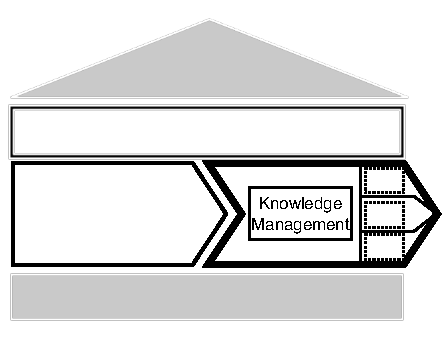
\includegraphics{figures/processes/knowledgemanagement.pdf}
		\end{center}
	\end{subfigure}

	\begin{subfigure}[b]{.32\textwidth}
		\begin{center}
			\begin{tikzpicture}
			[node distance=.5cm, minimum height=4.5em, start chain=going below,font=\sffamily]
			\node[punktchain, rounded corners=0pt , minimum height=2.8em,join=by {-}] (eins)      {maintain case master data};
			\node[punktchain,rounded corners=0pt, minimum height=2.8em,  join=by {-}] (zwei) {consolidate case data };
			\node[punktchain, rounded corners=0pt, minimum height=2.8em, join=by {-}, ] (drei) {combine case data};
			\node[punktchain, rounded corners=0pt, minimum height=2.8em, join=by {-}, ] (vier) {provide case data };

			\end{tikzpicture}
			\caption{Case-related variant}\label{fig:knowmang:case}
		\end{center}
	\end{subfigure}
\begin{subfigure}[b]{.32\textwidth}
	\begin{center}
		\begin{tikzpicture}
		[node distance=.5cm, start chain=going below,font=\sffamily]
		\node[punktchain, rounded corners=0pt, minimum height=2.8em,join=by {-}] (eins)      {maintain customer master data};
		\node[punktchain,rounded corners=0pt,  
		minimum height=2.8em,join=by {-}] (zwei) {consolidate customer data};
		\node[punktchain, rounded corners=0pt,  
		 minimum height=2.8em,join=by {-}, ] (drei) {combine customer data};
		\node[punktchain, minimum height=2.8em, rounded corners=0pt, join=by {-}, ] (vier) {provide customer data};
	
		\end{tikzpicture}
				\caption{Customer-related variant}\label{fig:knowmang:cust}
	\end{center}
\end{subfigure}
\begin{subfigure}[b]{.32\textwidth}
	\begin{center}
		\begin{tikzpicture}
		[node distance=.5cm, start chain=going below,font=\sffamily]
		\node[punktchain, rounded corners=0pt,minimum height=2.8em ,join=by {-}] (eins)      {maintain transaction data};
		\node[punktchain,rounded corners=0pt, minimum height=2.8em , join=by {-}] (zwei) {consolidate transaction data};
		\node[punktchain, rounded corners=0pt, minimum height=2.8em, join=by {-}, ] (drei) {combine transaction data};
		\node[punktchain, rounded corners=0pt , minimum height=2.8em,join=by {-}, ] (vier) {provide transaction data};
		
		\end{tikzpicture}
				\caption{Transaction-related variant}\label{fig:knowmang:trans}
	\end{center}
\end{subfigure}
	
\end{figure}
	 
	%%%%%%%%%%
	\section{Management Processes}
	%%%%%%%%%%
	%%%%%%%%%%
	\subsection{Product Development}
	
	NSD vs SE vs SD
	
	SD: viewing it from the designer perspective
	
	
	
	
	\subsection{Portfolio Management}
	
	cooper
	
	\subsection{People Lifecycle Management}
	gross bord 98
		Investitionsziele: platz 2 personalentwicklung \citep{ccnet2016}, beschaffung platz 4
	\subsection{Workforce Management}
	variants: plan, control?
	Hier muss auch Qualitätskontrolle rein. Heißt aber eigentlich Personaleinsatzplanung
	
	%%%%%%%%%%
	%%%%%%%%%%
	\section{Client Processes}
	
	With respect to the other two process groups of the framework, the client  processes show the smallest domain specificity, as the outsourcing process and the agreement between provider and client stands in focus. \acrshort{CRM} encloses the services themselves, but it does not impact the B2B-relationship that forms around provider and client in order to establish the service transition. 
	
	The outsourcing process is described in different frameworks in literature. \citep{perunovic2007outsourcing} investigate in outsourcing theories that cover the process as a whole and synthesize a five step process. It occurs that the greater part of frameworks take the outsourcing client's perspective, so that processes like \textit{vendor selection} or the alike are often part of frameworks. \citep{Agarwal_2008} present a rather neutral framework that is not fit on the role of the client and names activities that are driven by client and provider. \citep{deloittehandbook}, as practitioners, provide a comprehensive handbook for clients that is build around a six step process. 
	
	As the provider's perspective is taken in this thesis, the presented frameworks need to examined in terms of their applicability. Activities prior to signing of an outsourcing contract are either driven by internal analysis in the client organization whether outsourcing is a beneficial means or an external analysis of the available providers (vendors) on the market \citep{Franceschini_2003}. It is common practice to issue a \acrfull{RFP} to considered providers that mark the engagement of a relationship between the provider and the client. The following B2B-sales process ends with a signed contract between both parties that is followed by the service realization. This is chosen to be modeled in a single \textit{Sales} process (\cf \Fig \ref{fig:outsourcingprocess}), as the split into multiple components is motivated by (client)-internal steps prior to the approach of potential vendors. Providers can engage in pre-sales activities that may invoke the submission of a \acrshort{RFP} in the first place, but this pro-active sales approach can be seen as an optional part at the beginning of the sales process.
	
	The realization of the outsourcing agreement can be split into two streams, as seen in \citep{Agarwal_2008}. On the hand there is the creation of the provider's solution that addresses the client's problem. The solution relates to the provider's product portfolio and it's application on the case.  On the other hand, the client needs to pass over the existing in-house business to the provider in order to realize the outsourcing. These two aspects are separated into the two processes \textit{Solution Design} and \textit{Transition}. The former ends with the implementation of the service for the client, while the latter is completed with the takeover. The interdependency of these two is visualized by their parallel arrangement. 
	
	The last part of the examined outsourcing frameworks characterizes activities that take place after the transition is completed. From a provider perspective, this follow-up can be described as client relationship maintenance \citep{Moncrief_2005}. However, this wording would lead to confusion, as the target of the outsourcing activity (\viz \acrshort{CRM}) is not explicitly named on the framework. Due to this the related notion of \textit{Account Management }is chosen to represent this process, which emphasizes the B2B-aspect. 
	
	\begin{figure}[caption={Outsourcing process framework comparison}, label={fig:outsourcingprocesses}]
		{	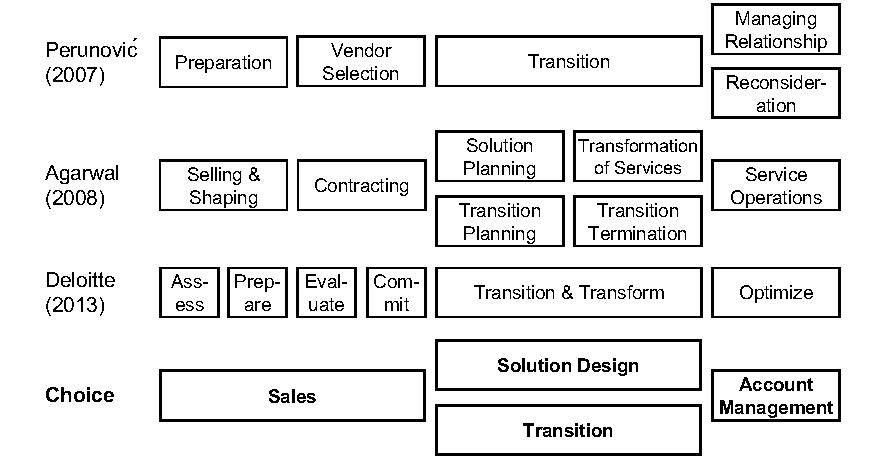
\includegraphics[width=.95\textwidth]{figures/outsourcingprocs.pdf}}
	\end{figure} 
	
	
	\subsection{Sales}
	
	This process marks the starting point of an outsourcing life cycle of a provider with a client. Building on a review existing paradigms for B2B-selling processes in the literature \citep{_ge_2011}, a linear process known as the  \enquote{seven steps of selling} shall serve as a blueprint for the process structure here. 
	
	With roots in the 1920s, \citep{Moncrief_2005} reviews the traditional seven steps and focuses on its applicability towards relationship selling, which aims at the \enquote{securing, building, and maintaining long-term relationships with profitable customers} \citep[\p{13}]{Moncrief_2005}. The technological progress has impacted the steps significantly, which is why the wording is to be accepted with reservation. The steps are (1) Prospecting, (2) Preapproach, (3) Approach, (4) Presentation, (5) Overcoming Objections, (6) Close, (7) Follow-Up. In contrast to the initial intent, the steps do not need to be sequentially completed and multiple people are involved instead of a single sales person. Moreover, it is abstracted from the physical meaning of \textit{approach} or \textit{presentation} for instance.
	
	\Fig \ref{fig:salesproc} shows the sales process and its detail processes are discussed in the following \wrt the steps of selling. Underlying process building blocks are not explicitly specified in this work, but suggestions for components are given in the textual description. 
	
	\begin{figure}[caption={Sales process}, label={fig:salesproc}]
		\begin{subfigure}[b]{.40\textwidth}
			\begin{center}
				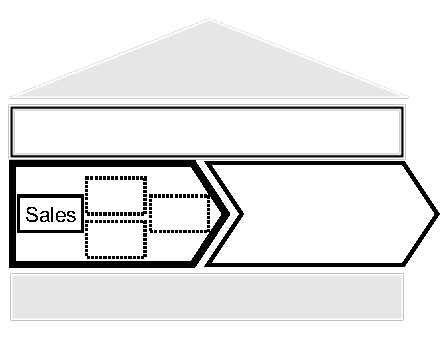
\includegraphics{figures/processes/sales.pdf}
			\end{center}
		\end{subfigure}
		\begin{subfigure}[b]{.9\textwidth}
			\begin{center}
				\begin{tikzpicture}
				[node distance=.5cm, start chain=going below,font=\sffamily]
				\node[punktchain, rounded corners=0pt, join=by {-}] (eins)      {identify prospect};
				\node[punktchain, rounded corners=0pt, join=by {-}] (zwei) {approach prospect};
				\node[punktchain, rounded corners=0pt, join=by {-}, ] (drei) {evaluate \acrshort{RFP}};
				\node[punktchain, rounded corners=0pt, join=by {-}, ] (vier) {create offer};
				\node[punktchain, rounded corners = 0pt, minimum height=2.6em,] (fuenf) {negotiate contract};
				\node[punktchain, left = of fuenf, minimum height=2.6em, rounded corners = 0pt,] (sechs) {perform due diligence};
				\node[punktchain, right = of fuenf, minimum height=2.6em, rounded corners = 0pt,] (sieben) {create commercial deal};
				\node[punktchain, below = of fuenf, rounded corners = 0pt,] (acht) {create contract};
					\draw[|-,-|,-, thick,] (vier.south) |-+(0,-0.5em)-| (fuenf.north);
					\draw[|-,-|,-, thick,] (vier.south) |-+(0,-0.5em)-| (sechs.north);
					\draw[|-,-|,-, thick,] (vier.south) |-+(0,-0.5em)-| (sieben.north);
						\draw[|-,-|,-, thick,] (fuenf.south) |-+(0,-0.5em)-| (acht.north);
					\draw[|-,-|,-, thick,] (sechs.south) |-+(0,-0.5em)-| (acht.north);
					\draw[|-,-|,-, thick,] (sieben.south) |-+(0,-0.5em)-| (acht.north);
				\end{tikzpicture}
			\end{center}
		\end{subfigure}
	
\end{figure}
	
	\subsubsection{Identify prospects}
	In order to enable a pro-active client approach in the selling process, the market has to be analyzed so that potential prospects can be targeted by the provider. It corresponds to the first step of selling (Prospecting), while the efforts towards a specific prospect can be seen as part of the pre-approach. 
	A prospect can be \enquote{ regarded [...] as a potential customer, client, \etc} \citep{oxfordprospect} and the provider's perception is that this organization can benefit from outsourcing processes. This activity requires the screening of in-house services, so that added-value for can be worked out. As there is no internal information (for example about costs) available at this point, this detail process is especially important in scenarios where the \acrshort{BPO} provider sees its strengths in providing a better service over solely cost reduction. The prospect might not be aware of the efforts of the provider and might not consider outsourcing as an option. Hence, the provider can expand its market and bring itself in an advantageous position in the following contact with the client. 

	
	\subsubsection{Approach prospects}
	
	Building on the market analysis that brought out a prospect, this step describes the provider's \textit{approach} towards the potential client, so that the provider can communicate its ideas. Clearly, this describes the third step of selling. The prospect can evaluate these and form a clearer picture of the circumstances, as the provider's ideas must base on assumptions due to lack of internal information. In the positive case, the prospect creates a bid, which represents the intent of a prospect to engage in outsourcing of a specified process. Considered providers are contacted and receive an \acrshort{RFP}. 
	
	The hitherto described two detail processes of selling can be seen as optional. If a client contacts a provider self-motivated, the process starts with the evaluation of the \acrshort{RFP}.
	
	\subsubsection{Evaluate \acrshort{RFP}}
	
	The third detail process has no direct reference to selling process, but represents a review of the received \acrshort{RFP}\footnote{Technically, there is a \acrfull{RFI} that is issued to a wider audience to receive first information from potential bidders \citep{bitkom2008}. However, responding to a \acrshort{RFI} does not show clear commitment from the provider.}. This is due to the fact that in the selling process, the willingness of the selling party is not in question. However, in the domain of outsourcing, a matching between client needs and offered services by the provider is necessary in order to establish a win-win situation. Furthermore, the action of issuing the \acrshort{RFP} (initiated by the prospect) requires a \textit{reaction} of the provider. This reaction needs to consider the requirements of the prospect internally in order to decide whether to participate in the bid. This evaluation examines the fit to the provider's service offerings, its sales strategy, but also macro-environmental factors of the bid. The PEST-framework \citep{0314852336} illustrates these as a mnemonic for political, economic, social and technological aspects that surround and influence the decision of an provider. 
	When the provider decides to continue the sales activity, the following process step, namely the creation of an offer is started. 
	
	\subsubsection{Create offer}
	The fourth detail process of sales describes the activities that are done to respond  to the client's \acrshort{RFP} by means of an offer. The corresponding fourth step in the selling (presentation), describes the presentation as the demonstration of the seller's products in terms of features, advantages and benefits \citep{Moncrief_2005}. This can also be implicitly seen in the offer, only that the boundaries are given by the \acrshort{RFP}. However, provider's need to make assumptions in the process. 
	
	As multiple providers receive an \acrshort{RFP}, there is competition. It is common for \acrshort{RFP} issuing companies to narrow down the candidates by creation of a \textit{short list} after reviewing the responses to the \acrshort{RFP}. This short list marks the next stage in the provider selection process, where more details are given to the remaining providers. In turn, these work in the new information to further specify the offer. As the final selection of a provider is a decision by the prospect, it is not further located in this process. 
	
	The following fifth part of the process is split into three parts in order to emphasize their connection to the fifth part of the steps of selling (overcoming objections). 
	
		
	\subsubsection{Negotiate contract}
	
	As the client\footnote{The contract describes a state where both parties have agreed to do outsourcing. Therefore, the term client is used instead of prospect from now on.} and provider move closer to an outsourcing agreement, both need to discuss terms and conditions. To capture mutual understanding, documents like a \acrfull{LOI} or a \acrfull{MOU} can be established.The contract is the legal formalization of the relationship between provider and the client \citep{Franceschini_2003}. 
	
	A \acrfull{SLA} describes \enquote{the performance level at which the service should be provided by the client} \citep[\p{32}]{deloittehandbook}. The contract specifies these to align the operational objectives of both parties and to incentivize correct behavior. Related to \acrshort{SLA}s is a credits regime, which specifies how performance below the \acrshort{SLA} is treated. 
	
	Covered aspects can be the operating model, process and scope, technology and tools, people, change management, transition planning, location management, security \& control, regulation or data privacy for instance \citep{deloittehandbook}. Aim of this detail process is to find an agreement, so that both parties are willing to set up and sign the contract.
	
	
	\subsubsection{Perform due diligence}
	
	Outsourcing can involve the transfer of personnel, hardware, software, contracts or licensing agreements for instance. The decrease of information asymmetries between provider and prospect helps the provider to compile a more detailed offer. Goal of due diligence is the systematic determination of all contents and related processes with respect to the outsourced services, so that there is a foundation to assess the project and its measures \citep[\p{13}]{bitkom2008}. This act of collecting knowledge minimizes risks by depending less on assumptions. This detail process aims at including more information from the client side in the sales process. 

	\subsubsection{Create commercial deal}
	
	The provider needs to develop a commercial model for its services that are subject to this outsourcing project. Financial engineering of the provider leads to a pricing model that needs to be agreed on\footnote{This agreement is reason for naming the object commercial deal instead of commercial model.}. The reader is referred to \ref{app:fineng} for typical pricing model elements. The activity of defining a commercial model is oriented towards the provider organization, which is reason for its explicit modeling \wrt client-oriented due diligence and bilateral negotiation detail process. 
	
	\subsubsection{Create contract}
	
	The sixth step of selling (close) describes the agreement of selling and buying party. In \acrshort{BPO} this document is represented by multiple contracts between provider and client. Previous negotiations, information from due diligence and the commercial deal are foundations for setup of the contracts. This detail process ends with the signing of the documents, which leads to the transition phase of the outsourcing life cycle. Usually there are separate contracts for outsourcing and the transition project \citep{bitkom2008}. 
	
	The seventh step of selling (follow-up) is represented in the Account Management process that covers the development of an existing outsourcing relationship. 
	
		
	\subsection{Transition}
	The objective of this process is to set the outsourcing into place by transition of work and resources. Transition\footnote{\enquote{The process or a period of changing from one state or condition to another.} \citep{oxfordtransition}} and transformation\footnote{\enquote{A marked change in form, nature, or appearance.} \citep{oxfordtransformation}} are two dominant terms in this phase. The former seems to have more popularity in literature \citep{perunovic2007outsourcing}, as its defining change aspect underlines the shift from the client to the provider. 
	
	The process, shown in \Fig \ref{fig:transproc}, is built around the transition plan object, which captures important steps during the transition project. It is noted that this plan needs to be conceptualized during contract negotiations and before signing the agreement, however \cite{deloittehandbook} list \textit{develop transition plan} as part of the transition phase. This intersection of the sales and transition process reasons their separation. The responsibility for the business is given to the provider in the \textit{transfer business} detail process, followed by knowledge transfer in the three dimensions of \acrshort{BPO}. 
	
	Three phases can be identified during the project \citep{bitkom2008, 0273705601}. In the \acrfull{PMO} phase the business is continued in an as-is state, while the following  \acrfull{TMO} phase implements changes. The objective is to reach the \acrfull{FMO}, that fulfills the requirements of the to-be state. However, this last phase is not part of the transition process, but normal operations. 
	
	\begin{figure}[caption={Transition process}, label={fig:transproc}]
		\begin{subfigure}[b]{.40\textwidth}
			\begin{center}
				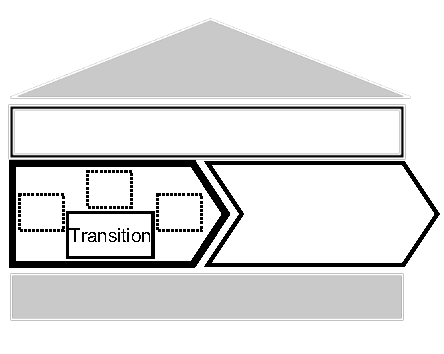
\includegraphics{figures/processes/transition.pdf}
			\end{center}
		\end{subfigure}
		\begin{subfigure}[b]{.9\textwidth}
			\begin{center}
				\begin{tikzpicture}
				[node distance=.5cm, start chain=going below,font=\sffamily]
				\node[punktchain, rounded corners=0pt, join=by {-}] (eins)      {develop transition plan};
	
		
				\node[punktchain, rounded corners=0pt, join=by {-}, ] (vier) {transfer business};
				\node[punktchain, rounded corners = 0pt,] (fuenf) {transfer process};
				\node[punktchain, left = of fuenf, rounded corners = 0pt,] (sechs) {transfer people};
				\node[punktchain, right = of fuenf,  rounded corners = 0pt,] (sieben) {transfer technology};
				\node[punktchain, below = of fuenf, rounded corners = 0pt,] (acht) {perform PMO phase};
				\node[punktchain, rounded corners = 0pt,join=by {-}, ] (neun) {perform TMO phase};
				\draw[|-,-|,-, thick,] (vier.south) |-+(0,-0.5em)-| (fuenf.north);
				\draw[|-,-|,-, thick,] (vier.south) |-+(0,-0.5em)-| (sechs.north);
				\draw[|-,-|,-, thick,] (vier.south) |-+(0,-0.5em)-| (sieben.north);
				\draw[|-,-|,-, thick,] (fuenf.south) |-+(0,-0.5em)-| (acht.north);
				\draw[|-,-|,-, thick,] (sechs.south) |-+(0,-0.5em)-| (acht.north);
				\draw[|-,-|,-, thick,] (sieben.south) |-+(0,-0.5em)-| (acht.north);
				\end{tikzpicture}
			\end{center}
		\end{subfigure}
		
	\end{figure}

	\subsubsection{Develop transition plan}
	Provider and client collaboratively develop a transition plan, that shows similarities to a project plan. A transition schedule, milestones and a work breakdown structure help to prepare both parties for the upcoming transition. Stakeholder commitment is important and a governance concept needs to be established for ensuring a frictionless course of action \citep{itgov2005}. The planning of work and especially knowledge transfer is another important aspect and linked to the project's success \citep{deloittehandbook}. 
	
	The completion of the transition plan marks the end of this detail process. While this step can start before completion of the sales process, the following activities represent the contract's execution and are consequently realized after an agreement of both parties. There is no explicit \textit{implement transition plan} detail process, because all of the following detail processes can be subsumed under this wording and thereby make it hardly expressive. 
	
	\subsubsection{Transfer business}
	
	The transfer of the business has the objective to bring the provider into control. One can also argue that this detail process must take place after underlying components (\ie people, process, technology) are transferred, so that details are specified before the provider is in charge. Another position can be that in order to orchestrate the components, knowledge about the entire business needs to be achieved. This perspective is preferred here and is reason for naming it the \textit{objective} of the detail process to take over control, so that knowledge transfer can take place before the responsibilities change. 
	
	Knowledge transfer is an important aspect and implicitly included in this and the following detail processes. A separate knowledge transfer detail process is not modeled, because it is seen as too unspecific for the transition step. Instead, the use of the verb \textit{transfer} shall emphasize its importance across the different dimensions. 
	
	The shift of the business to the outsourcing provider has to mind legal admissibility\footnote{In German law \cf §613a BGB }, that especially has implications on the transfer of staff. Moreover, the acquisition of tangible assets is to be handled. 
	
	\subsubsection{Transfer people, process, technology}
	
	Building on the people, process, technology split discussed in context of  \acrshort{BPO} in \acrshort{CRM} (\cf \ref{sec:proide}), each detail process emphasizes the respective aspect. In addition to the knowledge transfer that enables the provider to know \textit{how} the client organization has worked in the past \citep{perunovic2007outsourcing}, the provider has to integrate its own resources that enable an improvement over the status-quo.
	
	The training of existing staff towards new tasks or new personnel can be named in the \textit{people} dimension. The \textit{transfer process} step sets up new processes that are part of the service delivery. Lastly, \textit{technology transfer} establishes the compatibility of existing and new systems for service delivery. As these three aspects are closely related to the respective domain of the outsourcing (\viz \acrshort{CRM}), the solution from the provider is influencing at this point. While the design of the solution is located in a separate process, its outcome is integrated in this part of the transition process. 
	
	\subsubsection{Perform \acrshort{PMO} phase}
	The \acrshort{PMO}\footnote{Current Mode of Operation (CMO) is used synonymously. } phase starts with the transit of resources and responsibilities \citep{bitkom2008}. Its aim is to stabilize the business after shifting it to the provider. With respect to the transition plan, its duration is limited so that the intended changes can be performed shortly after in the \acrshort{TMO} phase.
	
	\subsubsection{Perform \acrshort{TMO} phase}
	After the as-is state is operating under the provider's responsibility, the implementation of changes can be initiated. The complexity of changes depend on the degree of innovation in the provided services \wrt as-is services. Reaching the \acrshort{FMO} phase ends this phase. With the service solutions in place, the regular \acrshort{SLA} and credit regime applies.
	
	\subsection{Solution Design}
	Deloitte: differentiate between service definition (\ie requirements) and service solution (how provider meets the requirements)
	\subsection{Account Management}